
%\mcom{I think the presence of \textbf{I} here is probably just noise: speaker variation w/r/t sensitivity to the negation effect. To be confirmed. \textbf{update:} it isn't noise.}
\chapter{Introduction}

In a 1999 monograph, \citeauthor{Bhat1999} posits a typological parameter along which languages variably assign prominence to \textsc{tense, aspect \textup{or} mood}. For Bhat, determining which of these grammatical macrocategories a given language appears to assign ``prominence'' gives rise to a number of generalisations about characteristics of that language's grammar (``correlatable characteristics''). In particular, he suggests that, in a language where $ \mathcal C $ is given prominence, notions belonging to the other two categories tend to be ``viewed in terms of $ \mathcal C $'' (7).


An important consequence of this typology, in which languages can be classified and differentiated on the basis of these three broad types, is the implication that languages can ``move between them'' --- that is observable, synchronic variation across this parameter points to a history of reanalysis of, for example, temporal categories as modal ones. While Bhat does not explore this consequence of his typology in detail, he does point to observations in the grammaticalisation literature that have demonstrated ``cross-categorial change'' --- that is, situations where lexical material denoting some temporal, modal or aspectual category come to be reanalysed conveying meaning about a category in another semantic domain. Bhat suggest, for example, that the well-attested alternative grammaticalisation trajectories described by \cite{Bybee1994} (among others) and represented in Figure \ref{ta-gram} are determined by the ``prominence'' that a given language accords to either temporal or aspectual distinctions \citeyearpar[182]{Bhat1999}. Of course, this treatment to some degree begs the question. In a given pair of related languages, what is it that underpins the change from, \textit{e.g.}, perfect marking to perfective marking for $ \mathcal L_1 $ versus past-tense marking in $ \mathcal{L}_2 $?

\begin{figure}[h] \caption{Two examples of attested meaning change between the aspectual and temporal domains}\centering\label{ta-gram}

\begin{subfigure}[b]{.45\textwidth}\caption{\gls{perf} grams develop into \gls{pfv} markers (\citealp[e.g.][]{Condoravdi2014} for Indo-Aryan) or \gls{pst} markers (\citealp[e.g.][]{Schaden2012} a.o.)}
		\begin{tikzpicture}[baseline=-2pt]
		\draw  (0,0) node(pf)  {\textcolor{forest}{\textsc{perf}}};
		\draw (1.75,.5) node(pv) {\textsc{pfv}};
		\draw (1.75,-.5) node(ps)  {\textcolor{red}{\textsc{pst}}};
		\draw[thick,->] (pf) -- (ps);
		\draw[->] (pf) -- (pv);
	\end{tikzpicture}
		\end{subfigure}\hfill
\begin{subfigure}[b]{.45\textwidth}\caption{\gls{prog} grams develop into \gls{ipfv} markers (\citealp[see][]{Deo2015a}) or \gls{pres} markers (\citealp[e.g.][]{Heinrichs2002} for Neo-Aramaic)}
		\begin{tikzpicture}[baseline=-2pt]
		\draw  (0,0) node(pg)  {\textcolor{forest}{\textsc{prog}}};
		\draw (1.75,.5) node(ip) {\textsc{ipfv}};
		\draw (1.75,-.5) node(pr)  {\textcolor{red}{\textsc{pres}}};
		\draw[->] (pg) -- (ip);
		\draw[thick, ->] (pg) -- (pr);
	\end{tikzpicture}
		\end{subfigure}
%\begin{tikzpicture}
%	content...
%\end{tikzpicture}
\end{figure}

\subsection{Futurity and mood-prominence}
Bhat marshalls data from Tibeto-Burman to show that ``mood-prominent'' languages have a tendency to grammaticalise a \textsc{future/nonfuture} distinction. He points to Manipuri, where this tense distinction appears to have `developed from an earlier realis-irrealis modal distinction' \citeyearpar[19]{Bhat1999}. The same verbal suffix \textit{-le} is a future tense marker in Manipuri, whereas \citet[67ff]{Bhat1999} shows that in related Mao Naga, it encodes irrealis modality, occurring in a number of modal, counterfactual and evidential constructions.


Additionally, going back to Aristotle, the truth of a future predication has frequently been analysed as changing with the passage of time ---- that is ```future contingent'' statements can be neither true nor false' \citep[265]{Thomason1970}. Consequently, these utterances about the future are often associated wth predictive illocutionary force. Contemporary formal treatments often embrace a modal semantics for ``future'' operators: one that departs from the earlier, priorian tense logic type approaches where truth is defined relative to time and --- the mirror image of \textsc{past} --- \textsc{future} is a sentential operator that serves to locate their prejacent subsequent to evaluation time.\footnote{This is not to suggest that Arthur Prior was unconcerned with this asymmetry between the future and the past --- indeed, over the course of his career he departs from an earlier belief in determinism and develops branching time models concerned with the indeterminate nature of the future. (\citealp[see][]{Copeland2020} and also \citealp[13]{Copley2009}). Generally speaking, on a deterministic view of the future, future morphemes can be unuderstood to universally quantify over an epistemic modal base, whereas on non-deterministic views they quantify over a metaphysical modal base.} Modal accounts of future, then, generally tend to take future-oriented morphology to universally quantify over a modal base. \citet[274]{Thomason1970} proposes that a the semantics of a future-tensed predication is as follows:\footnote{This following Copley's \citeyearpar[14]{Copley2009} conversion of \citeauthor{Thomason1970}'s account based on ``histories'' (which effectively imply sets of historical alternatives) into an equivalent one that speaks in terms of possible worlds. Thomason himself develops $ \mathcal{T\times W} $ frames in a \citeyear{Thomason1984} paper.}
\pex $ \denote[w,t]{\textsc{fut }p}=\left\{\begin{gathered}\begin{aligned} 1&\leftrightarrow &\forall w'\big[w'\simeq_t w \to \exists t' [t\prec t' \wedge p(w')(t')]\big]\\
0&\leftrightarrow &\forall w'\big[w'\simeq_t w \to \neg\exists t' [t\prec t' \wedge p(w')(t')]\big]
\end{aligned}\\
\text{undefined otherwise}\end{gathered}\right.
$\\[.5em]
\textsc{fut} $p$ is true if there's a time $ t' $ in the future of all metaphysical alternatives to $ w $ at $ t $ which $ p $ holds and false if there is no such time.\xe

Note that this semantics draws on the mechanics for futurity introduced in Ch. \ref{bambai} above. \textit{I.e.}, $\cup\simeq_t w $ is an equivalence class of worlds with identical histories to $ w $ up to $ t $ --- equivalent to Kratzer's \textit{metaphysical modal base}.

\subsection{Negation and mood}

Developing a broad cross-linguistic typology of sentential negation, \citet[208]{Miestamo2005} proposes a class of languages (\textsc{a/nonreal}) which have `grammaticalized the fact that negation belongs to the realm of the non-realized.' In many languages this means that a grammatical distinction between \textsc{realis} and \textsc{irrealis} modalities, drawn in positive clauses, is \textit{neutralised} in negative clauses. If irrealis markers are taken as operators which displace the instantiation of a given eventuality into the realm of the nonrealized, we can think of this semantic space as including or excluding negative declaratives. It is on these functional grounds that negation and mood interact; predicting parametric variation across languages.

%todo asymmetry. Muna participates (Bhat 67)


%\subsection{The semantics of a mood-based inflectional system}

. 


\subsection{Yolŋu Matha}

%Class of YM was discussed in Ch..... 
%To reorient the reader.....
%Djr, Wag are related....
%could move post-defense
Yolŋu Matha is a small language family spoken in North-Eastern Arnhem Land, in the Northern Territory of Australia. The family is a subgroup of the larger Pama-Nyungan family, representing something of an enclave in Northern Australia; surrounded by a diversity of unrelated languages.

\begin{figure}[h]
	\centering\caption{Traditional language communities in Northern Australia \citep{Horton1996}.Yolŋu Matha is the gold coloured area within the square in the primary map.\\\textbf{Inset. }Northeast Arnhem land (colourised from \citealt[2]{Wilkinson1991}. Yellow shading indicates the \textit{Yolŋu Wäŋa} (homeland). Brown and green circles indicate the contemporary distribution of Yolŋu languages investigated. Purple circling indicates the neighbouring (but genetically unrelated) Maningrida language family.}	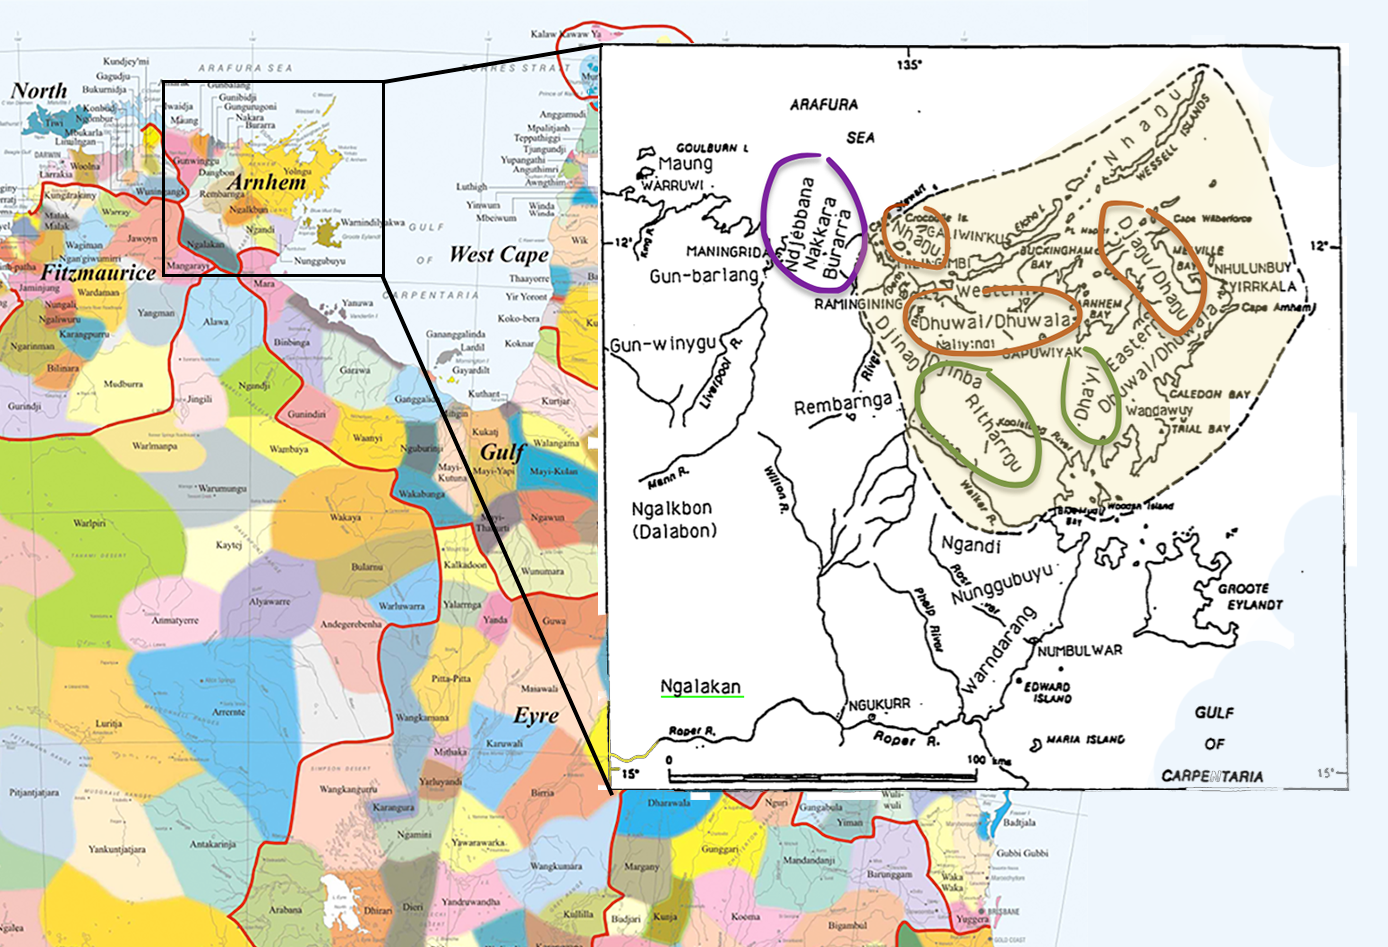
\includegraphics[width=0.9\textwidth]{AustralianLangsCropped.png}\label{map}
\end{figure}


Most Yolŋu linguistic phylogenies posit a high-level split between Western, Northern and Southern subgroups. This is schematised in Figure \ref{YM-phylo}. Yolŋu society is traditionally organised according to a moiety system --- \textit{Yirritja} and \textit{Dhuwa} --- and continues to be strictly exogamous with respect to moiety. Given that each Yolŋu clan is associated with a single patrilineal moiety and language variety, households are necessarily multidialectal, one member of a couple speaking a \textit{Yirritja} lect, the other speaking a \textit{Dhuwa} lect. This chapter focuses primarily on a number of Southern Yolŋu varieties (see Fig \ref{DDvars}).


\begin{figure}
\caption{A broad phylogenetic classification of Yolŋu subgroups, following \citealt{Wilkinson1991,Schebeck2001,Waters1989} a.o.}\centering\label{YM-phylo}
	\begin{tikzpicture}\tikzset{edge from parent/.style=
{draw,
edge from parent path={(\tikzparentnode.south)
-- +(0,-8pt)
-| (\tikzchildnode)}}}
		\Tree  [.\textbf{Yolngu~Matha} [.\textsc{Western} Djinang Djinba ] [.\textsc{Northern} Nhaŋu Dhaŋu-Djaŋu ] [.\textsc{Southern} \textit{Fig~\ref{DDvars}} ] ]
	\end{tikzpicture}
\end{figure}

\begin{figure}[h]\centering	\caption{Varieties (dialects) of \textcolor{teal}{Dhuwal}-\textcolor{ochre}{Dhuwala} in the context of the Southern Yolŋu languages \citep[following][13]{Wilkinson1991} with some adaptation following \citealt[15]{Schebeck2001}.}\label{DDvars}
	\begin{tikzpicture}[every node/.append style={align=right},every tree node/.style={anchor=north}]
		\Tree [.\textsc{\textbf{Southern~Yolŋu}} [.\textbf{\textcolor{ochre}{Ritharrŋu}-\textcolor{teal}{Wägilak}} $\vdots$ ] [ [.\textbf{Dhay'yi} $\vdots$ ] [.\textbf{Dhuwal-Dhuwala} [.\textsc{western} \node[text=teal,font=\itshape]{\bf\it Djambarrpuyŋu\\Ḻiyagalawumirr\\Ḻiyagawumirr\\Marraŋu}; \node[font=\itshape,text=ochre]{\bf\it Gupapuyŋu\\Wubulkarra}; ]   [.\textsc{eastern} \node[font=\itshape,text=teal] {Djapu\\Marrakulu\\Ḏäṯiwuy}; \node[font=\itshape,text=ochre]{Gumatj\\Maŋgalili\\Munyuku\\Maḏarrpa}; ] ] ] ]
	\end{tikzpicture}
	
\end{figure}\marginnote{right this is the classification in Wilk 91 which follows Dixon 80 presumably? Claire's phylogeny is different in a number of ways. how to handle?}

As indicated in the diagram, the \textit{Dhuwal} and \textit{Dhuwala} groupings effectively represent the distinct clan-lects of a single speech community --- associated with \textit{Dhuwa} and \textit{Yirritja} moieties respectively. Incidentally, \citet{Wilkinson1991} points out that the degree of similarity between Western Dhuwal and Dhuwala are more closely related to one another than either is to Eastern Dhuwal and Dhuwala (I assume that this fact is representable phylogenetically and has been represented in Figure \ref{DDvars}). The primary distinction between Dhuwal and Dhuwala varieties results from a productive apocope rule (\citealp[51]{Morphy1977}, \citealp[see also][94\textit{ff}]{Wilkinson1991} for further details.). The formal consequences of Dhuwal apocope on the verbal paradigm are partially indicated in parentheses in Table \ref{djr-pdm-exx} below. The table gives examples of the verb paradigm for each of the major Djambarrpuyŋu conjugation classes as described by \citet[306ff]{Wilkinson1991} (parentheses give the corresponding verb group number assigned by \citet{Lowe1996} for Gupapuyŋu.)


%\section{Dhuwal-Dhuwala: Djambarrpuyŋu \& Gupapuyŋu}\label{djr}



%todo §§4.1-4 to migrate directly in as descriptive background chapters
\section{Verbal inflection in Western Dhuwal(a)}\label{infls}



TMA distinctions in Dhuwal(a) are partially encoded in a paradigm that distinguishes four `inflections', which are cognate with a number proto-Yolŋu inflections according to the reconstructions provided by \citet{Bowern2009}. Work on Dhuwal and Dhuwala varieties (notably \citealt{Wilkinson1991,Lowe1996}) has tended to eschew a metalinguistic gloss for these inflections, given the ostensible non-unifiability of their semantics: the distribution of each of these inflectional categories is discussed in greater detail in what follows. In addition to these inflections, the labour of encoding TMA relations is shared by a (closed) class of auxiliaries, which appear to interact with the verbal paradigm. 




Further complicating the exposition of this, is the fact that there are a number of \textit{conjugation (sub)classes}: \citet{Lowe1996} identifies nine classes. The (more detailed) description by \citet{Wilkinson1991} shows that these correspond to three larger conjugation classes --- the \textit{Ø-}, \textit{N}- and \textit{Ŋ-}classes --- each associated with a number of subclasses,\footnote{\citeauthor{Wilkinson1991} appears to identify 14 distinct inflectional patterns in addition to a ``non-inflecting'' class (1991: 307).} in addition to ``non-inflecting'' and (semi-)irregular categories \citet{Wilkinson1991}. The paradigm for four WD verbs, taken to be representative of four different conjugation patterns is given in Table \ref{djr-pdm-exx}.

\mcom{Of course I can provide more detailed information (the subclasses) but that feels like it'd be better appended? The comparative spreadsheet i've made/Claire's 2009 stuff has most of this formative data... \\\textbf{note: Andrea Simms strongly suggests more exposition of the formal paradigm} }\begin{table}[h]\centering
	\begin{tabular}{rl|>{\it}l>{\it}l>{\it}l>{\it}l}
		\textbf{Class} & \textbf{\textit{Example}} & \textbf{I} & \textbf{II} & \textbf{III} & \textbf{IV}\\\midrule
		$\boldsymbol\emptyset_{i}$\hfill(2)& \textit{marrtji} `go' & \textit{marrtji}& \textit{marrtji} & \textit{marrtji\textbf{n(a)}} & \textit{marrtji\textbf{nya}}\\
		
		$ \boldsymbol\emptyset_{\textit{a}} $\hfill (3) & \textit{ḻuka} `consume' & \textit{ḻuk\textbf{a}} & \textit{ḻuk\textbf{i}} & ḻuka\textbf{n(a)} & ḻuka\textbf{nha}\\

		$\boldsymbol\emptyset_{\textit{rr}}$ \hfill (4)& \textit{waṉḏirr(i)} `run' & \textit{waṉḏi\textbf{rr(i)}}& \textit{waṉḏi} & \textit{waṉḏi\textbf{n(a)}} & \textit{waṉḏi\textbf{nya}}\\
		
		
		
		\textbf{N}\hfill(5)& \textit{ḻupthun} `wash' &\textit{ḻuphtu\textbf{n}} & \textit{ḻupthu\textbf{rr(u)}} & \textit{ḻupthu\textbf{rr(una)}} & \textit{ḻupthu\textbf{na}}\\
		
		\textbf{N$ _{L} $}\hfill(6)& \textit{gurrupan} `give' & \textit{gurrup\textbf{an}} & gurrupu\textbf{l(u)}&gurrupa\textbf{ra}& gurrupa\textbf{na} \\
		
		\textbf{Ŋ}\hfill(7)& \textit{nhäma} `see' & \textit{nhä\textbf{ma}} & \textit{nhä\textbf{ŋu}} & \textit{nhä\textbf{ŋal(a)}} & \textit{nhä\textbf{nha}}\\
	\end{tabular}
	\caption{Examples of the paradigm of four morphological TMA inflections in Djambarrpuyŋu [\gls{djr}] and (Gupapuyŋu [\gls{guf}] resyllabification in parentheses).\\{}[\gls{djr}] data and classification from \citet{Wilkinson1991}; [\gls{guf}] data and classification from \textit{Gupapuyŋu} \citeyearpar{Lowe1996}.} \label{djr-pdm-exx}
\end{table}


Above, I alluded to Beulah Lowe's eschewal of a ``semantic description'' for each of the four inflectional classes, also followed by Melanie Wilkinson. In the following subsections, I provide examples of the functional domains of each of the four inflections in Dhuwal-Dhuwala and other lexical material relevant to encoding TMA relations in this language. Throughout, these categories will be glossed with bold-faced Roman numerals, following the conventions established by Lowe (see also Table \ref{Infl-Comparisons-Wilk}, which adapts Wilkinson's summary of glossing decisions made by other grammarians.)% -- complex sentences and predications are investigated in further detail in §\ref{djr-subord}.

%Table \ref{Infl-Comparisons-Wilk}, adapted from \citet[336]{Wilkinson1991} summarises the metalanguage decisions made by other authors in their attempts to describe Dhuwal(a) varieties.

\begin{table}[h]
	\begin{tabular}{l|llll}
		&	\textbf{I}	& \textbf{II}	&	\textbf{III}	&	\textbf{IV}\\\midrule
		\citealt{Wilkinson1991} \gls{djr} &\textsc{First}&\textsc{Second}&\textsc{Third}&\textsc{Fourth}\\
		\citealt{Lowe1996} \gls{guf}\footnotemark &Primary&Secondary&Tertiary&Quartenary\\
		\citealt{Tchekhoff1983} \gls{djr}&\textsc{Bas}e&\textsc{Fut}ure&Past\textsubscript1&Past\textsubscript2\\
		\citealt{Heath1980} \gls{dwu} & Pres/Fut & Fut/Imp & Past & Past Remote\\
		\citealt{Morphy1983} (Djapu) & Unmarked & Potential & Perfective & Past Non-indicative\\
	\end{tabular}
	\caption{Summary of metalinguistic descriptors deployed by a number of grammarians for the four inflectional classes in a number of Dhuwal/Dhuwala varities, adapted from \citet[336]{Wilkinson1991}.}\label{Infl-Comparisons-Wilk}
\end{table}	\footnotetext{\citealt{VanderWal1992} adopts the same labelling scheme as \citealt{Lowe1996} although her analysis of the distribution of each category diverges somewhat.}


 Figure \ref{WilkDia} comprises a (colourised) reproduction of \citeauthor{Wilkinson1991}'s schematisation of the functional domain and collocation features of each Djambarrpuyŋu inflection. Data exemplifying the distribution of WD's four inflectional categories is provided in the subsections below in conjunction with a discussion of the approximate range of each.

\begin{figure}[h]\caption{Melanie Wilkinson's \citeyearpar[326]{Wilkinson1991} schematisation of the complex semantic space associated with each of the four inflectional categories in Djambarrpuyŋu. My colourisation.}\label{WilkDia}\centering
	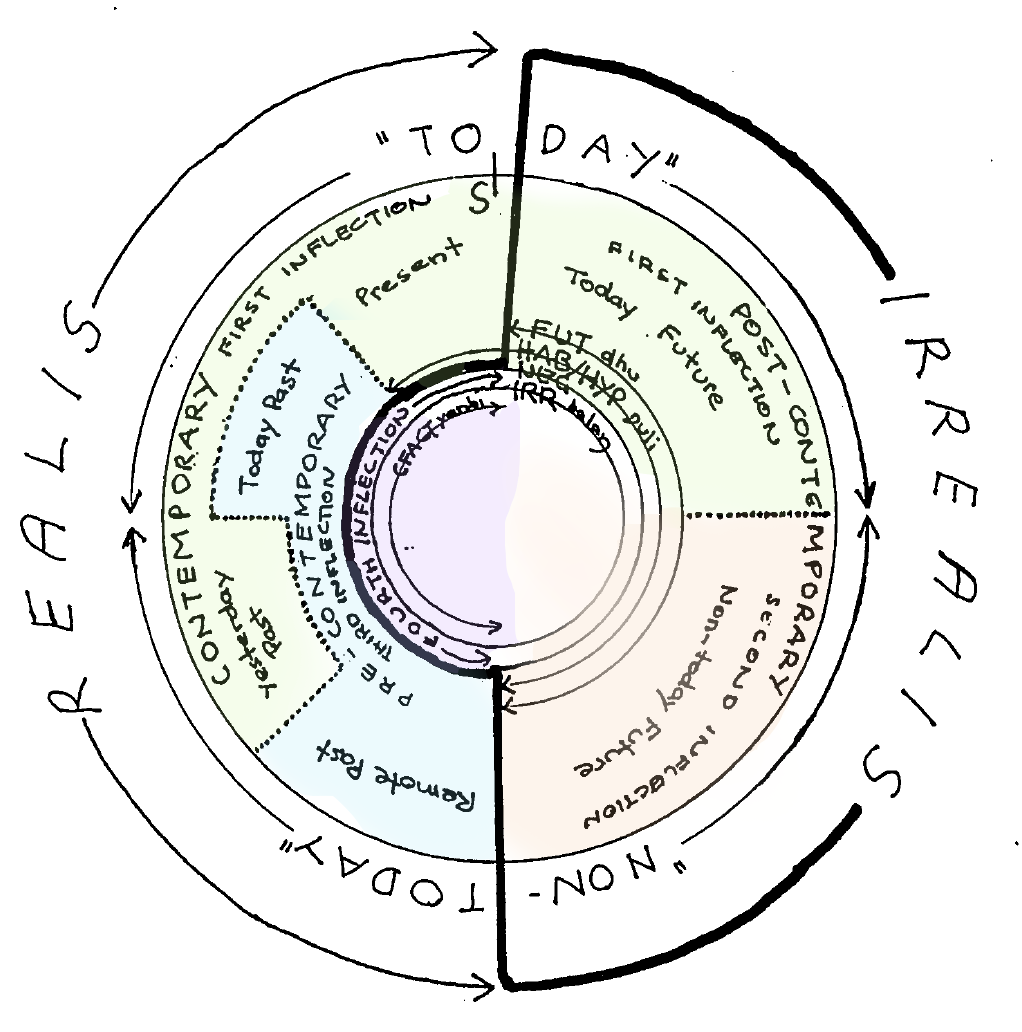
\includegraphics[width=0.8\textwidth]{WilkinsonDiagram362Col}
\end{figure}

\subsection{The Primary inflection}\label{desc-i}

The `primary' inflection (\textbf{I}), cognate with inflections in other Yolŋu languages which have been described as ``unmarked'' or ``base'', surfaces in predications about the present, past and future. Here I provide examples of \textbf{I}-inflected clauses receiving each of these temporal interpretations.

\mcom{Now for both of these (and i suspect all sentences in this sssection) context ought to be modulable s.t. a non-present reading is available. This can/should/will be tested in the field}\pex\textit{ Present-reference encoded with \textbf{I}}

\a\begingl\deftagex{IPres}\deftaglabel{nhina}
\gla Ŋunhi-y ŋunhi ḏirramu \textbf{nhina} ga//
\glb \gls{texd}\textsc{-erg} \textsc{texd} man sit.\textbf{I} \textsc{ipfv.\textbf{I}}//
\glft`There that man is sitting.'\trailingcitation{\citep[856]{Tchekhoff1983}}// 
\endgl
%\a\begingl \gla ŋarra \textbf{marrtji}-n dhiyaŋu-n bala//
%\glb 1s go\textbf{.I}-\gls{seq} \gls{prox}.\gls{erg}-\textsc{seq} then//
%\glft`I am going now.'\trailingcitation{\citep[256]{Wilkinson1991}}//\endgl
\a\begingl\gla Ŋarra ga \textbf{ḻuka} gapu (dhiyaŋu bala)//
\glb 1s \textsc{ipfv.\textbf{I}} consume.\textbf{I} water \gls{texd}.\gls{erg} then//
\glft`I'm drinking water at the moment.'\trailingcitation{[DhG 20190405]}//\endgl
\xe

The sentences given in (\getref{IPres}) show the compatibility between present temporal reference and the \textbf{I} inflection: in both cases, the event described by the predicate (\textit{nhina} `sit.\textbf{I}' and \textit{marrtji} `go.\textbf{I}') --- in both cases modified by the aspectual auxiliary \textit{ga} --- is understood as being contemporaneous with speech time. %todo Both sentences receive event-in-progress readings (also co-occurring with explicit aspectual marking, see §\ref{djr-asp} for more.)

%\mcom{Is it a shitty idea to use colour coding for more formatting/highlighting options? I want to reserve bold for the verbforms themselves but would like to be able to second-order emphasise non-paradigmatic things like TFAs, aspectual ops...}
\pex \textit{Past-reference encoded with \textbf{I}}\deftagex{pstI}

%\a\deftaglabel{nhama}\begingl\gla barpuru linyu \textbf{nhäma} dirramu-ny//
%\glb yesterday 2d see.\textbf{I} boy-\gls{acc}//
%\glft`Yesterday we saw a boy'\trailingcitation{\citep[569]{Tchekhoff1985}}//\endgl


\a\deftaglabel{ŋayatham}\begingl\gla ga \textbf{ŋayatham} ŋunha baṉ'thula-wuy ŋayambalk//
\glb and reach.\textbf{I} \gls{dist} \textsc{place}-\gls{assoc} place//
\glft`And (then we) reached the place (associated with) Baṉthula.'\trailingcitation{\citep[461]{Wilkinson1991}}//\endgl



\a\deftaglabel{rrupiya}\begingl\gla ḏirramu-wal yothu-wal bäpa-'mirriŋu-y rrupiya barpuru djuy'yu-\textbf{n} märr barpuru ga barpuru \textbf{buna}-ny dhiyal-nydja//
\glb man-\gls{obl} kid-\gls{obl} father-\gls{kinprop}-\textsc{erg} money yesterday send.\textbf{I} somewhat yesterday and yesterday arrive.\textbf{I}-\textsc{prom} \gls{prox}.\gls{erg}-\gls{prom}//
\glft`The father sent money to the boy recently and it arrived here yesterday'\trailingcitation{\citep[343]{Wilkinson1991}}//\endgl

\xe

In addition to those present-referring sentences in (\blastx), the data in (\getfullref{pstI}) show compatibility between \textbf{I} and past time reference. For both examples, the events described by the predicates (\textit{e.g.}, the seeing event described by \textit{nhäma} in (\getref{pstI.ŋayatham})) \textit{precede} speech time. Similarly, the two past events in (\getref{pstI.rrupiya}) both receive \textbf{I} inflection. The instantiation times of both of these events are restricted by the temporal frame adverb \textit{barpuru} $\approx$ `yesterday.% -- frame adverbials of this type are discussed in some detail in §\ref{TFA}.

Futher, the examples in (\getref{futI}) above, show the compatibility of \textbf{I}-inflected verb forms and \textsc{future }temporal reference.

\pex \deftagex{futI} \textit{Future-reference encoded with \textbf{I}}
\a\deftaglabel{lakaram}\begingl\gla yalala ŋarra dhu nhokal lakara-\textbf{m}//
\glb later 1s \textsc{fut} 2s\textsc{.obl} tell-\textbf{I}//
\glft `Later (today) I'll tell you.' \trailingcitation{\citep[373]{Wilkinson1991}}//\endgl

\a\deftaglabel{buna}\begingl \gla dhiyaŋ~bala walal dhu \textbf{buna}, yalala//
\glb now 3p \textsc{fut} arrive.\textbf{I} later//
\glft`They are coming later today.'\trailingcitation{\citep[256]{Wilkinson1991}}//\endgl


\a\begingl\glpreamble Deontic force with \textit{dhu}+\textbf{I} (see §\ref{dhu})//
\gla Way! Nhe dhu gurruka-\textbf{m} helmet! Rom ga \textbf{waŋa}.//
\glb Hey! 2s \gls{fut} wear-\textbf{I} \textit{helmet} law \textsc{ipfv.\textbf{I}}  say.\textbf{I}//
\glft`Oy! You wear a helmet! The law says so!\trailingcitation{[AW~20170730]}//\endgl

%\a\deftaglabel{marrtji}\mcom{Actually, W claims this is ``imminent action'' so we really just have a futurate use of \textbf{I} without \textit{dhu} (interesting data point in itself) This can probably move to the section on future marking (either \textbf{I} or \textbf{\textit{dhu}})}\begingl\glpreamble `Imminent action' without \textit{dhu}//
%\gla \ljudge{$ ^{\%*} $}ŋarra marrtji-n \textbf{dhiyaŋu}-n \textbf{bala}//
%\glb 1s go-\gls{seq} \textbf{\gls{prox}.\gls{erg}}-\gls{seq} \textbf{\gls{mvtawy}}//
%\glft`I'm going now.'\trailingcitation{\citep[256]{Wilkinson1991}}//\endgl

\xe


 In both sentences, the event described by the predicate is understood to obtain in the \underline{future} of speech time (modulo additional constraints on imminence/immediacy described below). %\mcom{Evidence of infelicity of \textit{dhu}-less future readings? I actually kinda doubt on the basis of Tonnhauser, Bohnemeyer's work that this is going to be a hard constraint}
  In these sentences the presence of \textsc{fut} marker \textit{dhu} is apparently obligatory in order to establish future reference. %(Although according to \citet[256]{Wilkinson1991} (\getfullref{futI.marrtji}), a futurate interpretation is ostensibly available. This use is unavailable to Ramingining speakers.

\subsection{The Secondary inflection}\label{desc-ii}

Like \textbf{I}, the Secondary inflection (\textbf{II}) has a range of uses. It is notably obligatory when predicating of future times \underline{beyond the current day} and is the main strategy for forming \underline{imperative sentences}.

\pex\deftagex{futII} \textit{Future-reference encoded with \textbf{II}}
\a\deftaglabel{lakaraŋ}\begingl\glpreamble Co-occurring with \textit{dhu} `\gls{fut}'//
\gla yalala-ŋu-mirri-y ŋula~nhätha ŋarra dhu nhokal lakara\textbf{-ŋ}//
\glb later-\textit{ŋu}-\gls{prop}-\gls{erg} sometime 1s \textsc{fut} 2s-\gls{obl} tell-\textbf{II}//
\glft`I'll tell you sometime later on'\trailingcitation{\citep[346]{Wilkinson1991}}//
\endgl
%\a\deftaglabel{nhini}\begingl\glpreamble Future interpretation independent of \textit{dhu} `\gls{fut}'//
%\gla ŋayi boŋguŋ \textbf{nhini} \textbf{ŋäku} ŋarra-ny ŋunhal yirrkala//
%\glb 3s tomorrow sit.\textbf{II} hear.\textbf{II} 1s-\gls{prom} \gls{dist}-\gls{loc} \textsc{placename}//
%\glft`She'll be there at Yirrkala tomorrow, listening to me'\trailingcitation{\citep[340]{Wilkinson1991}}//\endgl

\a\begingl\glpreamble Infelicity of \textbf{I} with non-today future//
\gla Barpuru goḏarr ŋarra dhu nhä(\textbf{-ŋu/$^*$-ma})//
\glb funeral tomorrow 1s \gls{fut} see(-\textbf{II}/$^*$-\textbf{I})//
\glft `I'll see the funeral tomorrow'\trailingcitation{[AW~20180730]}//\endgl

\xe

The two sentences in (\getref{futII}) show how \textbf{II} is used in concert with the particle \textit{dhu} to establish future temporal reference.
% The conditions on the (non-)appearance of \textsc{fut}-marker \textit{dhu} are unclear at the present time (see §\ref{dhu} for more), but future-readings with \textbf{II} do not appear to be reliant on this auxiliary (cf. the data in (\getref{futI}) above).
  A notable contrast between (\getfullref{futI.lakaram}) and (\getfullref{futII.lakaraŋ}) is the apparently obligatory retrieval of a \textsc{today}-reference time for \textbf{I}-inflected futures, as against a (probable) \textsc{beyond-today}-reference time for \textbf{II}-inflected futures.\footnote{\citet[347]{Wilkinson1991} gives an example of a speaker using a \textit{dhu}-\textbf{II} structure in the context of a narrative she is telling, signalling that she `will (return to the time of the old people).' Wilkinson takes this as evidence of an association between \textbf{II} and the irrealis. This generalisation is pursued in detail in this chapter.} Effectively, this distinction seems to be one place where the grammar of Dhuwal(a) grammaticalises ``temporal remoteness'' (\citet{Comrie1985,Dahl1985} referred to elsewhere in the literature as ``metrical tense'' \citealp[e.g.][204]{Chung}).\footnote{Although \citet[39]{Heath1980} suggests of the \textbf{II} future in Dhuwal Proper (his \textsc{Fut/Imp}) that this form encodes a type of ``normative nuance'' (a clear extention of imperative flavour into future assertions.)}


(\getref{irrII}) shows the compatibility of \textbf{II} with a (future-oriented) possibility reading. Modal particles including \textit{balaŋ(u), ŋuli} and \textit{bäynha} are responsible for the `weakening' or `downtowning' of the speaker's commitment to the prejacent proposition. 
%Modal operators are described in §\ref{modals}.

%\mcom{It would be good to get sentences with richer context (i.e. an established time of instantiation for the prejacent (tomorrow, imminently etc...)) 
%	This said we can probably assume that the we're talking about immediate future here... Is \textbf{I} incompatible with this? There's not much more to say here until I have speaker judgments on this question.}
\pex\a\deftagex{irrII}\begingl\gla Ŋarra ŋuli \textbf{bäynha} dhiŋgu-\textbf{ŋ} ŋawulul-yu//
\glb 1s \textsc{hyp} \textsc{mod} die-\textbf{II} smoke-\textsc{erg}//
\glft`I might die from the smoke.'\trailingcitation{\citep[164]{Buchanan1978}}//\endgl
\a\begingl\gla ŋayi bala \textbf{balaŋu} bukthu-\textbf{rru}//
\glb 3s \gls{mvtawy} \gls{irr} break-\textbf{II}//
\glft`It (the recorder) might break.'\trailingcitation{[DG~20190417]}//\endgl
\xe



\textbf{II} is additionally used to encode imperative clauses (\getref{impII}). Shown in (\getfullref{impII.proh}), negative imperatives (probibitives) are treated identically.\footnote{Although, as discussed in Ch. \ref{NEC} (see also Phillips ms. `Negation (in Australian Languages)') the use of privative-marked nominals is another common, more ``indirect'' strategy.}

\pex\textit{Imperative force with \textbf{II}}\deftagex{impII}
%\a\begingl\gla g...y, ḻupmara-\textbf{ŋu}-n ŋarra-ny//
%\glb \textsc{name} wash-\textbf{II}-\gls{seq} 1s-\gls{prom}//
%\glft`G...y, wash me!'\trailingcitation{\citep[360]{Wilkinson1991}}//\endgl

\a\begingl\gla wäy! gurtha ŋunha, nhawi, ḏutji män-\textbf{ŋu}, bakmara-\textbf{ŋu}//
\glb hey! fire(wood) \gls{dist} what's.it firesticks get-\textbf{II} break\textbf{-II}//
\glft`Hey! Get that firewood, what's it, those firesticks, and break them.'\trailingcitation{\cite[114]{VanderWal1992}}//\endgl

\a\deftaglabel{proh}\begingl\gla yaka walala-ŋ buku-bakamara-\textbf{ŋ}//
\glb \gls{neg} 3p-\gls{dat} head-break-\textbf{II}//
\glft `Don't answer them!'\trailingcitation{\citep[360]{Wilkinson1991}}//\endgl


\a\begingl\gla nhä\textbf{-ŋu} nhanŋu dhurrwara!//
\glb look-\textbf{II} 2s.\gls{dat} door//
\glft`Look at her mouth!'\trailingcitation[AW 20180731]//\endgl

\xe




\subsection{The Tertiary inflection}\label{desc-iii}

The Tertiary inflection (\textbf{III}) is generally associated with predications about the \textsc{past}. An important caveat, however, is that this inflection is \ul{infelicitous when describing \textsc{recent} events instantiated \textsc{before the current day}.} The examples in (\nextx) below show the compatibility between \textbf{III} and a reference time that is `earlier today.'\mcom{Show the compatibility of \textbf{III} with \gls{ipfv} by adding some examples with \textit{gana}. (Perhaps a minimal pair, though this might be better placed below.)}

\pex \textit{\textsc{Today past} and the \textbf{III} inflection}\deftagex{pstIII}
\a\deftaglabel{gathur}\begingl\gla Gäthur ŋayi \textbf{marrtjin} räli Galiwin'ku-ŋur//
\glb today 3s go.\textbf{III} hither \textsc{place}-\gls{abl}//
\glft`[Earlier] today he came from Galiwin'ku.'\trailingcitation{\citep[150]{Buchanan1978}}//\endgl

\a\deftaglabel{bili}\begingl\gla Bili ŋayi \textbf{marrtjin} dhipuŋur natha-ŋur nyan'thuna-ŋur//
\glb \textsc{compl} 3s go.\textbf{III} \textsc{prox.abl} food-\gls{abl} eat.\textbf{IV}-\textsc{abl}//
\glft`He has already gone from having lunch here.'\trailingcitation{\citep[150]{Buchanan1978}}//\endgl


\a\begingl\glpreamble Infelicity of \textbf{III} with \textsc{recent past}//
\gla barpuru ŋarra nhä\textbf{(-ma/*-ŋala)} ḏetuŋ//
\glb yesterday 1s see\textbf{(-I/$^\#$-III)} buffalo//
\glft`I saw a buffalo yesterday.'\trailingcitation[MD 20180802]//\endgl

\a\begingl\glpreamble Infelctity of \textbf{I} with \textsc{today past}//
\gla gathura ŋarra nhä\textbf{($^\#$-ma/-ŋala)} ḏetuŋ dhukarra-ŋura//
\glb today 1s see\textbf{$ ^\# $-I/III} buffalo road-\gls{loc}//
\glft `I saw a buffalo down the road today'\trailingcitation{[MD 20180802]}//
%\textsc{comment.} Event could have happened this morning or ten minutes before speech time.//\
\endgl
\xe

\mcom{Potentially look for a ref for this or provide data that makes this unambiguous...}
(\getfullref{pstIII.gathur}) shows the compatibility between temporal frame adverbial (TFA) \textit{gäthur(a)} `today' and \textbf{III} in \gls{djr}, which leads to an temporal interpretation of `earlier today.'\footnote{Note however that the reckoning of \gls{tfa} \textit{gäthur(a)} differs to that of English and other familiar languages as shown in (\getfullref{neg-pst.munha}), where \textit{gäthur munhawa} `today nighttime' is interpreted as ``last night'' and still triggers \textbf{III} marking on the verb.} However even in the absence of a \gls{TFA}, the event described in (\getref{pstIII.bili}) is interpreted as having been instantiated \textsc{earlier.today}/in the immediate past of speech time. Nonetheless, as the data in (\nextx) show \textbf{III} cannot be properly described as a `hodiernal past.' 


\pex\textit{\textsc{Remote past} and the \textbf{III} inflection}\deftagex{remIII}

\a\deftaglabel{wawa}\begingl\gla nhä nho-kiyin-gal wäwa-'mirriŋu-y warkthu-rr ŋäthil rarrandharr-yu//
\glb what 2s-\textsc{emph}-\gls{obl} bro-\gls{kinprop}-\gls{erg} work-\textbf{III} before dry~season-\gls{erg}//
\glft`What did your brother do last summer?'\trailingcitation{\citep[343]{Wilkinson1991}}//\endgl

\a\deftaglabel{malwan}\begingl\glpreamble\textsc{context.} The speaker is describing a locality as it was in her youth.//
\gla märrma' ga-\textbf{n} malwan-dja dhärra-\textbf{n} yindi maṉḍa-ny//
\glb two \textsc{ipfv}-\textbf{III} hibiscus-\gls{prom} stand-\textbf{III} big 3d-\gls{prom}//
\glft`Two big hibiscus flowers were (growing).'\trailingcitation{\citep[339]{Wilkinson1991}}//\endgl

\a\deftaglabel{wuŋgan}\begingl\glpreamble\textsc{context.} A man is telling a story from long ago . His friend's dog has spotted a water goanna.//
\gla ...ŋunhi wurkaḏi-y nhä-ŋal-{na} ŋinya dharpa-lil-a ŋal'yu-na nhäwi wan'kawu-ya//
\glb \gls{texd} \textsc{name}-\gls{erg} see-\textbf{III} 3s.\gls{acc} tree-\gls{all}-\gls{seq} ascend-\textbf{III} whatsit water.goanna-\gls{ana}//
\glft`\textit{Wukaḏi} watched it scramble up into a tree, the water goanna.'\trailingcitation{\citep[193]{Heath1980}}//\endgl
%todo >>>>> \marginnote{I've taken some liberties with the glossing here, Heath has the second verb \textit{ŋal'yuna} as \textbf{I} with a \textsc{seq} marker... to investigate further perhaps}



\xe


Unlike the \textsc{hodiernal} temporal interpretations that the sentences in (\blastx) receive, the two sentences in (\lastx) are evaluated to obtain in the `\textsc{remote past}.' In (\getfullref{remIII.wawa}),\mcom{may be easier just to get a similar non-interrogative sentence to do what \lastx b does} the instantiation time of the predicate is restricted by two frame adverbials: \textit{ŋäthil(i)}, which picks out a time `in the distant past; prior to/earlier than (some other time)' \citep[158]{Wilkinson1991} and \textit{rarrandharryu} `dry season':\footnote{The suffix \textit{-Thu} (\textit{-yu} as a postsonorant allomorph), glossed here as \gls{erg} is used to mark ergative NPs as well as instrumental (\gls{instr}) NPs and to form TFAs out of nominals \gls{temp}.} The cooccurrence of these expressions restricts the predicate being questioned to \textit{a prior dry season}. Conversely, the declarative sentence in (\getfullref{remIII.malwan}) requires no adverbial specification. A \textsc{remote past} interpretation arises as a result of the \textbf{III} inflection alone, which is precised pragmatically by the discourse context (\textit{sc.} a narrative that the speaker is telling about her childhood.) (\getref{remIII.malwan}) will be able to retrieve a same-day past interpretation as well, with sufficient contextual support.

%\mcom{This discussion of the Maningrida treatments of ``frame'' and ``tense'' may be better placed • entirely in the lit. review, • after the general data discussion of inflections, or • in the following chapter.} 
The ostensible `discontinuity' of the times that predicates receiving \textbf{I} and \textbf{III} inflection can refer to has been described in preceding literature as \textbf{\textsc{cyclic time reference}} \citep[88]{Comrie1983}. In her treatment of Burarra [\gls{bvr}], \citet{Glasgow1964} draws a distinction between `tense' and `frame of reference' (`timescale' for \citealt[48]{Green1987}). The interaction between these is, in effect, taken to give rise to a reference interval. This analysis has been adopted and developed by others working on Maningrida languages (\citet[165]{Eather2011} for Nakkara [\gls{nck}], \citet{Green1995} for Gurr-goni [\gls{gge}] and \citet{McKay2000} for Ndjébanna [\gls{djj}].) The interpretation of interacting ``tense'' morphology and reference frames is schematised in Table \ref{GlaswegianTR}. 
%todo The following chapter further treats and formalises this analysis.



\begin{table}[h]\centering\onehalfspacing
	\begin{tabular}{@{}llll@{}}\toprule
		
		&                 & \multicolumn{2}{c}{\textsc{frame}}          \\ 
		&                 & \multicolumn{1}{c}{\textbf{today}}         & \multicolumn{1}{c}{\textbf{before today}}      \\\midrule
		\multirow{2}{*}{\textsc{\rotatebox[origin=c]{90}{infl}}} & \textbf{\phantom{I}I}    & now           & yesterday/recently \\
		& \textbf{III} & earlier today & long ago           \\ \bottomrule%(l){2-4} 
	\end{tabular}
	\caption{A \citealt{Glasgow1964}-style analysis of \textbf{past-time restrictions} introduced by the verbal inflections, adapted for the Dhuwal(a) data. \textbf{I} and \textbf{III} inflections correspond to Eather's \textbf{contemporary} and \textbf{precontemporary} ``tenses'' (``precontemporary'' is Eather's \citeyearpar[166]{Eather2011} relabelling of Glasgow's ``remote'' tense.)}\label{GlaswegianTR}
\end{table}
%\mcom{Also the get sick/psych/phys condition verbs, some examples also in Buchanan:168}

%todo %%%%%% this is on psych verbs / stative verbs and lexical aspect.
%Additionally, a set of psychological predicates that are frequently translated into English as present-tensed stative verbs appear with \textbf{III}. Examples are given in (\nextx).
%
%
%\pex\deftagex{psychPreds}\a\begingl\gla ŋarra dhuwal/dhika djawaryu-\textbf{rr}/rerrikthu-\textbf{rr}/djanŋarrthi-\textbf{n}//
%\glb 1s \textsc{prox/indefp} be.tired-\textbf{III}/be.sick-\textbf{III}/be.hungry-\textbf{III}//
%\glft`I'm (a bit) tired/sick/hungry'\trailingcitation{\citep[278]{Wilkinson1991}}//\endgl
%\a\begingl\gla bili djawar'yu-\textbf{rr}-a//
%\glb \gls{cplv} be.tired-\textbf{III}//
%\glft`They're already tired'\trailingcitation{\citep[365]{Wilkinson1991}}//\endgl
%\mcom{Needs elicitation work, appears to be a today-past thing? Are these predicates available with TFAs \textit{barpuru?}, with \textit{ga}? And the other inflections??\\
%	Test entailments also: \textit{??I was tired this morning but i'm not now??}}
%\a\deftaglabel{nhaŋal}\begingl\gla ŋarra dhu dhuwal lakara-m ƞunhi nhä ŋarra nhä-\textbf{ŋal} dhiyaŋ bala//
%\glb 1s \gls{fut} \gls{prox} tell-\textbf{I} \gls{texd} what 1s see-\textbf{III} \gls{prox}.\gls{erg} \gls{mvtawy}//
%\glft`I'll tell you what I see right now.'\trailingcitation{\citep{Wilkinson1991}}//\endgl
%\xe
%
%\citet[365-6]{Wilkinson1991}, in effect, suggests that the frequent exponence of \textbf{III} in these predicates of ``emotional and bodily states'' is a function of their lexical semantics. Unlike their English translations, with \textbf{III}, these predicates can be understood as `achievements' (to borrow from Vendler's Aktionsart taxonomy). In these cases then, \textbf{III} is licensed because \textit{djarwaryu\textbf{rr(u)}} refers to a state-change before speech time. Consequently, the licensing of \textbf{III} in (\getfullref{psychPreds.nhaŋal}) above is a consequence of a completed \textit{seeing} eventuality immediately prior to the \textit{telling}-event described in the matrix clause. This phenomenon is investigated in detail in §\ref{anY}\texttt{.1?} below.


\subsection{The Quaternary inflection}\label{desc-iv}


%\mcom{Is this XLinguistic note worth anything? If so a couple more examples would be nice.}
The Quartenary inflection (\textbf{IV}) has a broad range of uses in Dhuwal(a) varieties that correspond in part to categories described in Australian languages including \textit{past potentialis} \citep{Heath1980a}, \textit{past counterfactual} \cite{McKay2011}, \textit{[past] irrealis} \citep[159]{Austin1998} \textit{etc.} It co-occurs with modal auxiliaries (especially \textit{ŋuli} `\gls{hab}' and \textit{balaŋ(u)} `\gls{irr}') in order to describe past habituals (\getref{habIV}) and hypothetical/counterfactual descriptions as in (\getref{hypIV}).


\pex\a\deftagex{habIV}\begingl\gla Ŋayi \textbf{ŋuli} märra-\textbf{nha} ŋunhi meṉḏuŋ-nha//
\glb 3s \gls{hab} get-\textbf{IV} \gls{texd} snail-\gls{acc}//
\glft`She would (used to) get (collect) snails'\trailingcitation{\citep[147]{Buchanan1978}}//\endgl

%todo \mcom{check ft for (b)} <<<<——— nusure what this note wouldve been about.
\a\begingl\gla ...ŋorra-\textbf{nha} walal \textbf{ŋuli} marrtji-\textbf{nya} ŋunhi-li-yi, galku-\textbf{na} walal \textbf{ŋuli} ga-\textbf{nha} gapuw wirwiryu-\textbf{na}+ra-w//
\glb lie-\textbf{IV} 3p \textsc{hab} go-\textbf{IV} \textsc{texd}-\gls{loc}-\gls{ana} wait-\textbf{IV} 3p \textsc{hab} \textsc{ipfv}-\textbf{IV} water-\gls{dat} turn-\gls{nmlzr}-\gls{dat}//
\glft`They would be lying there, they would be waiting for the water to stir.'\trailingcitation{(DB Djon 5:4)}//\endgl
\a\begingl\gla waṯuy \textbf{balaŋu} ḻuka-\textbf{nha} chocolate//
\glb dog.\gls{erg} \gls{irr} eat-\textbf{IV} chocolate//
\glft`The dog could've/must've eaten the chocolate.'\trailingcitation{[DG~20190413]}//\endgl

\xe

\pex\a\begingl\glpreamble\deftagex{hypIV}\textsc{context.} Speaker had a toothache.//
\gla barpuru balaŋ ŋarra bala dentist-kal marrtji-\textbf{nya} dhiyak//
\glb yesterday \textsc{irr} 1s \gls{mvtawy} dentist-\gls{obl} go-\textbf{IV} \gls{prox}-\gls{dat}//
\glft`Yesterday I should have gone to the dentist for a filling'\trailingcitation{\citep[353]{Wilkinson1991}}//\endgl

\a\begingl\gla Yaka balaŋ nhe marrtji-\textbf{nya} Darwin-lil//
\glb \gls{neg} \textsc{irr} 2s go.\textbf{IV} Darwin-\gls{all}//
\glft`You should not go to Darwin.'\trailingcitation{\citep[164]{Buchanan1978}}//\endgl\xe


These data demonstrate the relationship between the \textbf{IV} inflection and combinations of past temporal reference and various modal and aspectual operators. 


\subsection{Summary}

As mentioned above, a number of authors have eschewed assigning a metalinguistic label to the four inflectional categories that are realised on Western Dhuwal verbs. This due to the data's apparent resistance to an analysis where each marker realises some unified semantic category (\textit{i.e.}, \textsc{past, present} etc.) Wilkinson's diagramatic representation of the relevant semantic categories and how they are partitioned by the inflectional system is repreoduced as Figure \ref{WilkDia}.




Ultimately, a consequence of this distribution gives rise to a phenomenon which \citet[83]{Comrie1985} refers to as ``cyclic tense'' : where a given verbal inflectional category appears to be licensed by ``discontinuous intervals.'' These licensing intervals are schematised in Figure \ref{TempSchem}. On the basis of these data, a formalisation of the observations made by \citealt{Glasgow1964} \textit{et seq.} (those summarised in Table \ref{GlaswegianTR}) can be represented as (\nextx) below, where the domains of each of these inflections are discontinuous intervals.\footnote{\textsc{note} that the disjunctive semantics given in (\getref{disjunct}) is not intended to represent a proper treatment of these inflectional categories in Djambarrpuyŋu. This is a topic of current and ongoing work which is sadly out of the scope of the current dissertation.} $ \textit{today}:\mathcal T\to\wp(\mathcal T) $ is that function which returns the interval spanning from the beginning until the end of the day of utterance.\footnote{The basics of this treatment of temporal metricality (or ``remoteness'') converge to some degree with \citeauthor{Cable2013}'s 2013 proposal for Gikũyũ tense and \citeauthor{Klecha2016} on Luganda tense.}




\begin{figure}[h]\caption{Past-time temporal expression in the Yolŋu Matha varieties of Central Arnhem, demonstrating two descriptive phenomena: (a) cyclicity --- the interspersion/discontinuity of \textbf{I} and \textbf{III} forms and (b) metricality --- the (subjective) division of the past domain between these two forms.\\$\lfloor{\sl today}\rfloor$ indicates the boundaries of the day of utterance. $\boldsymbol{t*}$ is utterance time.}\label{TempSchem}\centering
		\begin{tikzpicture}[scale=1.2]
		% draw horizontal line   
			\draw[<->, line width=.5mm] (0,0) -- (12,0);
%		\draw[<-, line width=.5mm] (0,0) -- (9.5,0);	
		%draw rex
		\shade[left color=blue!15!white, right color=green!15!white] (0,0.02) rectangle (4.8,1.5);
		%	\fill[green!10!white] (2.5,0.02) rectangle (4.8,1.5);
		\fill[blue!10!white] (4.8,0.02) rectangle (6.8,1.5);
		\fill[green!10!white] (6.8,0.02) rectangle (9.5,1.5);
			\fill[orange!10!white] (9.5,0.02) rectangle (12,1.5);
		
		% draw nodes
		\draw (1.25,0) node[below=3pt] {\textbf{}} node[above=10pt] {\textsc{\textbf{III}}};
		\draw (3.675,0) node[below=3pt] {\textbf{}} node[above=10pt] {\textbf{I}};
		\draw (5,0)   node[circle,fill,label={below,align=left}:$\big\lfloor{\sl today}$] {} node[below=3pt] {\textbf{}} node[above=3pt] {};
		\draw (6.8,0) node[diamond,shade,outer color=black, inner color  = ochre,label=below:$\boldsymbol{t*}$] {} node[below=3pt] {\textbf{}} node[above=3pt] {\textsc{}};
		\draw (5.8,0) node[below=3pt] {\textbf{}} node[above=10pt] {\textsc{\textbf{III}}};	
		\draw (8.15,0) node[below=3pt] {\textbf{}} node[above=10pt] {\textsc{\textbf{I}}};	
			\draw (10.75,0) node[below=3pt] {\textbf{}} node[above=10pt] {\textsc{\textbf{II}}};	
		\draw (9.5,0)   node[circle,fill,label=below:${\sl today}\big\rfloor$] {} node[below=3pt] {\textbf{}} node[above=3pt] {};
		
		
		%%%braces
		
		\draw [decorate,decoration={brace,amplitude=4pt},xshift=-0pt,yshift=35pt]
		(0.5,0.5) -- (4.5,0.5) node [black,midway,yshift=0.35cm] 
		{\footnotesize metricality};
		
		\draw [decorate,decoration={brace,amplitude=4pt},xshift=-0pt,yshift=40pt]
		(3.5,0.5) -- (9,0.5) node [black,midway,yshift=0.35cm] 
		{\footnotesize cyclicity};
		
	\end{tikzpicture}
\end{figure} 


\pex\textbf{A polysemy treatment of the temporal contribution of \textbf{I} and \textbf{III} (to be rejected)}\deftagex{disjunct}
	\a$\llbracket\textbf{\phantom{I}I\phantom{I}}\rrbracket^{c}=\lambda P\lambda t\!*.\exists t'\begin{cases}t\in today\leftrightarrow t\succeq t*&.\,P(t')\qquad\textsc{[nonpast]}\\
	t\prec today \leftrightarrow \mu(t,t*)<s_c&.\,P(t')\qquad\textsc{[recent past]}
\end{cases}$

\textbf{I} asserts that $ P $ holds at $ t $ where:\\
\textbf{\textsc{either}} the reference time $ t$ doesn't precede speech time $ t*$,\\ \textbf{\textsc{or}} if $ t $ \textsc{precedes}  $ today $, then the temporal distance by which $ t $ precedes $ t* $ is \textit{\textbf{below} some contextually provided standard} $ s_c $

\a$\llbracket\textbf{III}\rrbracket^{c}=\lambda P\lambda t\!*.\exists t'\begin{cases}t\in today\leftrightarrow t'\prec t*&.\,P(t')\qquad\textsc{[today past]}\\
	t\prec today \leftrightarrow\mu(t',t*)>s_c&.\,P(t')\qquad\textsc{[remote past]}
\end{cases}$

\textbf{III} asserts that $ P $ holds at $ t $ where: \\
\textbf{\textsc{either}} the reference time $ t $ falls within $ today $, in which case it precedes speechtime $ t* $,\\ \textbf{\textsc{or}} if $ t $ \textsc{precedes} $ today $, the temporal distance by which $ t $ precedes $ t* $ is \textit{\textbf{above} some contextually provided standard} $ s_c $
\xe


%%%%PRESUPP/REFERENTIAL
%\pex\textbf{A polysemy treatment of the temporal contribution of \textbf{I} and \textbf{III}}\deftagex{disjunct}
%\a$\llbracket\textbf{\phantom{I}I\phantom{I}}\rrbracket^{c}=\lambda t:\begin{cases}t\in today\leftrightarrow t\succeq t*&.\,t\qquad\textsc{[nonpast]}\\
%	t\prec today \leftrightarrow \mu(t,t*)<s_c&.\,t\qquad\textsc{[recent past]}
%\end{cases}$
%
%\textbf{I} enforces a presupposition that:\\
%\textbf{\textsc{either}} the reference time $ t $ doesn't precede speech time $ t*$,\\ \textbf{\textsc{or}} if $ t $ \textsc{precedes}  $ today $, then the temporal distance by which $ t $ precedes $ t* $ is \textit{\textbf{below} some contextually provided standard} $ s_c $
%
%\a$\llbracket\textbf{III}\rrbracket^{c}=\lambda t:\begin{cases}t\in today\leftrightarrow t\prec t*&.\,t\qquad\textsc{[today past]}\\
%	t\prec today \leftrightarrow\mu(t,t*)>s_c&.\,t\qquad\textsc{[remote past]}
%\end{cases}$
%
%\textbf{III} enforces a presupposition that: \\
%\textbf{\textsc{either}} the reference time $ t $ falls within $ today $, in which case it precedes speechtime $ t* $,\\ \textbf{\textsc{or}} if $ t $ \textsc{precedes} $ today $, the temporal distance by which $ t $ precedes $ t* $ is \textit{\textbf{above} some contextually provided standard} $ s_c $
%\xe


\subsection{Cyclic tense}

While the lexical entries given in (\lastx) are descriptively adequate, they are also arbitrary and disjunctive. Here, I will claim that \I{} and \III{} differ because \III{} (compatible with strictly past temporal reference) presupposes that \textbf{non-final instantiation} (\textsc{nfi}) of its prejacent \citep[cf.][]{Condoravdi2014}. 

\begin{figure}[h]
	\centering	\caption{Appealing to `nonfinal instantiation' to provide a unified entry for the temporal reference of \textbf{III}}\label{NFI}
	
	\begin{tikzpicture}
		\draw[<->, line width=.5mm] (0,0) -- (12,0);
		\draw[line width=.8mm,densely dotted] (5,1.8) -- (5,-1.8); 
		\draw[line width=.8mm,densely dotted] (9,1.8) -- (9,-1.8);
		\draw[line width=2mm,nearly transparent] (7.35,1.8) -- (7.3,-1.8) node [at end,yshift=-2mm] {\textit{\textsc{now}}};
		
		
		\filldraw[nearly transparent,green](3,0)		ellipse [x radius=2cm,y radius=1cm];
		\draw (2.25,.25) node[color=blue] {\textbf{$ k $}};
		\filldraw[nearly transparent,blue,xshift=0.2cm](2,0)		ellipse [x radius=1.2cm,y radius=.6cm];
		\draw (4.25,.25) node[color=forest] {\textbf{$ i $}};
		\filldraw[nearly transparent,green,xshift=.28cm](6,0)		ellipse [x radius=1.2cm,y radius=.8cm];
		\draw (7.3,.25) node[color=black] {\textbf{$ i $}};
		\filldraw[nearly transparent,blue,xshift=.15cm](6,0)		ellipse [x radius=1.05cm,y radius=.5cm];
		\draw (6,.25) node[color=blue] {\textbf{$ k $}};
		
		
		\fill[very nearly transparent,ochre] (9.5,1) -- (9.5,-1) -- (11.5,-1) -- (11.5,1); 
		
		
		
		\draw [decorate,decoration={brace,amplitude=6pt},xshift=-0pt,yshift=40pt]
		(5.1,0.5) -- (9,0.5) node [black,midway,yshift=0.35cm] 
		{\footnotesize \textsc{today}};
		
		\draw [decorate,decoration={brace,amplitude=6pt},xshift=-0pt,yshift=40pt]
		(0,0.5) -- (4.9,0.5) node [black,midway,yshift=0.35cm] 
		{\footnotesize \textsc{before}};
		
		\draw [decorate,decoration={brace,amplitude=4pt},xshift=-0pt,yshift=20pt]
		(3.5,0.5) -- (4.8,0.5) node [black,midway,yshift=0.35cm] 
		{\footnotesize \textit{barpuru}};
		
		\draw [decorate,decoration={brace,amplitude=4pt},xshift=-0pt,yshift=20pt]
		(0.5,0.5) -- (3,0.5) node [black,midway,yshift=0.35cm] 
		{\footnotesize \textit{baman'}};
		
		\draw [decorate,decoration={brace,amplitude=4pt},xshift=-0pt,yshift=20pt]
		(9.25,0.5) -- (11.8,0.5) node [black,midway,yshift=0.35cm] 
		{\footnotesize \textit{goḏarr'}};
		
	\end{tikzpicture}
	
\end{figure}

Context makes available two possible reference intervals $ i_c $: \textsc{today} and \textsc{pre-today}. \III~situates its prejacent within a nonfinal subinterval of $ i_c $. The infelicity of \textbf{I}-inflected predicates with \textsc{remote} and \textsc{today past} instantiation times then emerges as a result of pragmatic blocking. It is well demonstrated that oppositions between specific and general meanings give rise to a division of pragmatic labour in which the general form is conventionally restricted to the complement of the domain of the specific form (\citealp{Deo2015}, citing \citealp{Horn1984} \& \citealp{Horn2012a}).

\pex\textbf{An NFI-based attempt at a lexical entry for the \textsc{third} inflection}

$ \denote[g,c]{\textbf{III}} = \lambda P\lambda i_c:\exists j[j\underset{\textsc{final}}{\sqsubseteq} i_c.\textsc{NfInst}(P,i_c,j)]$\\
The context makes available either a \textsc{today} or \textsc{pretoday} interval $ i_c $. \III~presupposes the existence of a final subinterval $ j $. \III~ asserts that $ P $ is instantiated at some subinterval of $ i $ that wholly precedes $ j $ (i.e. that \textsc{NfInst}($ P,i_c,j $) holds.)

\xe


%\subsection{So what about \II~ and \IV?}

Meanwhile, as demonstrated above, \textbf{II} and \textbf{IV} both appear to co-occur with modal particles. Predications about the future (beyond the day of utterance $ today $) obligatorily occur with \textit{dhu} `\gls{fut}' and receive \textbf{II} inflection. As shown in \S\ref{desc-ii}, however, \textit{dhu}+\textbf{II} can also receive a range of modal necessity readings; suggesting a treatment of \textit{dhu} as a circumstantial modal.\footnote{In view of the range of readings available to \textit{dhu}, \citet[110]{VanderWal1992} glosses this particle as \gls{mod}.}

So far, we have only considered ``positive'' clauses. In the section that follows, we see how the picture of WD inflection we have developed here complexifies significantly under negation.

\section{Sentential negation: \textit{yaka} \& \textit{bäyŋu}}\label{negs}

Discussed in Ch. \ref{NEC-yolŋu}, Djambarrpuyŋu has two negative particles, \textit{yaka} and \textit{bäyŋu}, both of which are deployed for standard negation (\textit{i.e.} those particles whose effect is to reverse the truth value of a given proposition.) The primary distributional distinction between these is that only \textit{yaka} is used to generate negative imperatives (prohibitives) whereas only \textit{bäyŋu} is found in negative existential/quantificational contexts. Both of these sentential negators, however, interact with verbal inflection.


Descriptively, as shown in the data in (\getref{neg-pres}-\getref{neg-pst}), negation appears to trigger a ``switch'' from the `realis-aligned inflections' (\textbf{I}~and~\textbf{III}) to their `irrealis counterparts', (\textbf{II}~and~\textbf{IV}) which otherwise turn up predominantly in hypothetical or counterfactual contexts. Effectively, this evinces a reality status-based distinction that is neutralised in negated sentences \citep[see also][356]{Wilkinson1991} for Western Dhuwal(a). This is schematised below in Table \ref{negneut}.

\begin{table}[h]\centering
	\begin{tabular}{ccc}
		&\multicolumn{2}{c}{\textsc{\textbf{polarity}}} \\
		& \textsc{--neg} & \textsc{+neg}\\\midrule
		&	\textbf{I} & \multirow{2}{*}{\textbf{II}}\\
		& \textbf{II} \\\midrule
		&	\textbf{III} & \multirow{2}{*}{\textbf{IV}}\\
		& \textbf{IV} \\\bottomrule
	\end{tabular}
	\caption{Neutralisation of \textbf{I} and \textbf{III} inflections under negation.}\label{negneut}
\end{table}


The following examples in (\getref{neg-pres}) show how sentences that receive \textbf{I}-marking in positive sentences --- encoding temporal reference to the present or recent past --- instead receive \textbf{II}-marking under the scope of negation. Each example contains a predications about the present or about the recent past, each receiving \textbf{II}-marking under negation. (a-b) presents a near-minimal pair, where a predicate with present reference ``switches'' inflection from \textbf{I} to \textbf{II} under negation.s

\pex\textit{Exponence of present and recent past reference as \textbf{II} under negation}
\deftagex{neg-pres}


\a\begingl%\glpreamble Present-tensed sentence with \textbf{I}//
\gla Nhaltja-\textbf{n} \textbf{ga} limurru-ŋgu-ny rom waŋ-\textbf{a}?//
\glb do.how-\textbf{I} \gls{ipfv}.\textbf{I} 1p.\gls{incl}-\gls{dat}-\gls{prom} law say-\textbf{I}//
\glft`What does our law say?'\trailingcitation{(DB~Luk~14.3)}//\endgl

\a\begingl%\glpreamble Negated present-tense sentence receives \textbf{II} marking//
\gla \textbf{yaka} \textbf{gi} \textbf{biyak} rom waŋ-\textbf{i}//
\glb \textbf{\gls{neg}} \gls{ipfv}.\textbf{II} do.thusly.\textbf{II} law say-\textbf{II}//
\glft`That's not how the law is/what the law says.'\trailingcitation{\citep[357]{Wilkinson1991}}//\endgl 




\a\begingl%\glpreamble  Negated present-tense sentence receives \textbf{II} marking\\\textsc{context.} Speaker is trying to read from a computer screen.//
\gla \textbf{bäyŋu} ŋarra \textbf{gi} nhä-\textbf{ŋu}//
\glb \textbf{\gls{negq}} 1s \gls{ipfv}.\textbf{II} see-\textbf{II}//
\glft`I can't see (it).'\\
%\textsc{comment.} \textit{nhäŋu} (`see.\textbf{II}') could also mean yesterday in past.
\textsc{\textbf{comment.}} `I didn't see (it) (yesterday)' also available.\trailingcitation{[AW 2018030]}//\endgl



\a\begingl\gla Ŋarra gi bäyŋu maḻŋ'mara-\textbf{ŋu} waṯu (ŋarraku). Bili ŋayi ga nhin-\textbf{a} wäŋaŋura//
\glb 1s \textsc{ipfv}.II \gls{neg} appear.\gls{caus}-\textbf{II} dog 1s.\gls{dat} \gls{cplv} 3s \gls{ipfv} sit.\textbf{I} house.\gls{loc}//
\glft`I can't find my dog. It lives in the house.'\trailingcitation{[DG~20190417]}//\endgl



\a\begingl\gla Ŋarra ga djäl-thi-rri giritjirrinyarawu, yurru ŋarra bäyŋu-nha \textbf{girritji}//
\glb 1s \gls{ipfv}.\textbf{I} want-\gls{vblzr}-\textbf{I} dance.\gls{nmlzr}-\gls{dat} but 1s \gls{neg}-\gls{seq} dance-\textbf{II}//
\glft`I was wanting to dance (at the \textit{buŋguḻ} yesterday) but I didn't dance (because I'd hurt my leg yesterday.)'\trailingcitation{[DG~20190417]}//\endgl
%\a\begingl\glpreamble\textsc{context.} A recent hunting trip, narrated in \textbf{I} for corresponding positive descriptions.//
%\gla ga \textbf{yaka} ŋayi ŋunhi dharyu-\textbf{rr} \textbf{biyak} djin'tjiŋdhu-\textbf{rr}//
%\glb and \textbf{\gls{neg}} 3s \gls{texd} rain-\textbf{II} do.thusly.\textbf{II} rain~lightly.\textbf{II}//
%\glft`...and it did not rain lightly'\trailingcitation{\citep[357]{Wilkinson1991}}/endgl
\xe


Similarly, in contexts where the temporal reference of the event description predicts that the verb will receive \textbf{III}-inflection --- that is the same-day or the remote past --- , when under the scope of a negative particle (\textit{yaka/bäyŋu}), the verb instead receives \textbf{IV}-inflection. This is shown by the data in (\getref{neg-pst}), where (a-b) represents a minimal pair, negative marking triggering the ``switch'' from \textbf{III} to \textbf{IV} inflection. (c) shows the negation of an immediate past event licensing \textbf{IV} inflection, (d) shows how a negated, \textbf{IV}-inflected predicate can be embedded under a propositional attitude predicate to encode a false belief, and (e) an example of a negated description of the remote past receives \textbf{IV} inflection.

\pex \textit{Exponence of \textsc{today past} and \textsc{remote past} reference as \textbf{IV} under negation}\deftagex{neg-pst}
%\a\deftaglabel{munha}\begingl\gla bäyŋu ŋarra gäthur ŋorra-\textbf{nha} manymak-ku-\textbf{nha} munhawu//
%\glb \gls{negq} 1s today lie-\textbf{IV} good-\gls{tr}-\textbf{IV} nighttime//
%\glft`I didn't sleep well last night'\trailingcitation{\citep[357]{Wilkinson1991}}//\endgl

%\mcom{Though the second clause in (b) also has ŋuli so maybe this is not quite so nice an ex. as originally thought}\a\begingl\gla ŋäthil-nydja ŋarra ga-n dhuwal, ga miltjiri marrtji-n \ bäyŋu ŋarra ŋuli ga-\textbf{nha} nhä-\textbf{nha}//
%\glb earlier-\gls{prom} 1s \gls{ipfv}-\textbf{III} \gls{prox} and blind go-\textbf{III} \textbackslash \gls{negq} 1s \gls{hab} \gls{ipfv} see-\textbf{IV}//
%\glft`I was blind before; I was unable to see'\trailingcitation{\citep[358]{Wilkinson1991}}//\endgl


\a\begingl\gla gathur munhagumirr ŋarra nhä-\textbf{ŋal} warrakan//
\glb today morning 1s see-\textbf{III} bird//
\glft`I saw a bird this morning'\trailingcitation{[FW 20180802]}//\endgl


\a\begingl\gla gathur munhagumirr \textbf{bäyŋu} ŋarra nhä-\textbf{nha} warrakan//
\glb today morning \textbf{\gls{negq}} 1s see-\textbf{IV} bird//
\glft`I didn't see a bird this morning'\trailingcitation{[FW 20180802]}//\endgl

\a\begingl\glpreamble \textsc{\textbf{context}.} Speaker has dropped a coin.//
\gla Way! \textbf{Bäyŋu} ŋarra nhä-\textbf{nha}?//
\glb Hey! \textbf{\gls{negq}} 1s see-\textbf{IV}//
\glft`Ah! Did you see (it)?'\trailingcitation{[AW 20180830]}//\endgl


\a\begingl\glpreamble\textbf{\textsc{context.}} I'm at work explaining to my coworker why my \textit{galay} is angry at me.//
\gla Ŋarraku miyalk maḏakarritj-thi-na bili ŋayi ga guyaŋa ŋarra ga-\textbf{nha} bäyŋu djäma//
\glb 1s.\gls{dat} wife anger-\gls{inch}-\textbf{III} \gls{cplv} 3s \gls{ipfv}.\textbf{I} think.\textbf{I}\footnotemark{} 1s \gls{ipfv}-\textbf{IV} \gls{neg} work//
\glft`My wife got angry because she thought I wasn't working today.'\trailingcitation{[DG~20190417]}//\endgl

\a\begingl\glpreamble \textbf{\textsc{context.}} The speaker grew up in the desert.//
\gla \textbf{bäyŋu} ŋarra ŋuli ganha nhä-\textbf{nha} (waltjaṉ) ŋunhi ŋarra yothu yän//
\glb \textbf{\gls{neg}} 1s 	\gls{hab} \gls{ipfv} see.\textbf{IV} rain \gls{texd} 1s child just//
\glft`When I was young, I hadn't seen [rain]/never saw [rain].'\trailingcitation{[AW~20190501]}//\endgl

%\a\begingl\glpreamble\textsc{context.} The text describes remote past events, narrated in \textbf{III} for corresponding positive descriptions//
%\gla ŋayi-ny muka bäyŋu yan yolŋu-ny yurrumdhu-\textbf{na}//
%\glb 3s-\gls{prom} okay \gls{negq} \gls{emph}  person-\gls{prom} gather-\textbf{IV}//
%\glft`Not all the people had gathered together'\trailingcitation{\citep[357]{Wilkinson1991}}//\endgl
\xe

The data in (\getref{neg-pres}-\getref{neg-pst}), demonstrate the interaction between temporal reference and negative polarity in WD, consistent with Miestamo's \textsc{a/nonreal} class --- the distinction between \textit{realized} and \textit{nonrealized} states of affairs is neutralised is negative contexts in WD. We can then provide a modified version of Figure \ref{TempSchem} to give the parallel diagram in Figure \ref{NegSchem}. The differences between these two diagrams schematise the effects of negation on the licensing of particular WD inflectional categories.

\begin{figure}[h]\centering\caption{Apparent interactions between temporal relations and reality status in Djambarrpuyŋu: cyclicty and metricality under negation.}\label{NegSchem}
	\begin{tikzpicture}[scale=1.2]
		% draw horizontal line   
		\draw[<->, line width=.5mm] (0,0) -- (12,0);
		
		%draw rex
		\shade[left color=violet!15!white, right color=orange!15!white] (0,0.02) rectangle (4.8,1.5);
		%	\fill[green!10!white] (2.5,0.02) rectangle (4.8,1.5);
		\fill[violet!10!white] (4.8,0.02) rectangle (6.8,1.5);
		\shade[left color=orange!10!white, right color=green!10!white] (6.8,0.02) rectangle (9.5,1.5);
		\fill[orange!10!white] (9.5,0.02) rectangle (12,1.5);
		
		% draw nodes
		\draw (1.25,0) node[below=3pt] {\textbf{}} node[above=10pt] {\textsc{\textbf{IV}}};
		\draw (3.675,0) node[below=3pt] {\textbf{}} node[above=10pt] {\textbf{II}};
		\draw (5,0)   node[circle,fill,label=below:$\lfloor{\sl today}$] {} node[below=3pt] {\textbf{}} node[above=3pt] {};
		\draw (7,0) node[diamond,shade,inner color=ochre,outer color=black,label=below:$\boldsymbol{t*}$] {} node[below=3pt] {\textbf{}} node[above=3pt] {\textsc{}};
		\draw (5.8,0) node[below=3pt] {\textbf{}} node[above=10pt] {\textsc{\textbf{IV}}};	
		\draw (7.5,0) node[below=3pt] {\textbf{}} node[above=10pt] {\textsc{\textbf{II}}};
		\draw (9,0) node[below=3pt] {\textbf{}} node[above=10pt] {\textsc{\textbf{I}}};	
		\draw (10.75,0) node[below=3pt] {\textbf{}} node[above=10pt] {\textsc{\textbf{II}}};	
		\draw (9.5,0)   node[circle,fill,label=below:${\sl today}\big)$] {} node[below=3pt] {\textbf{}} node[above=3pt] {};
		
		%		%braces
		%		\phantom{	\draw [decorate,decoration={brace,amplitude=4pt},xshift=-0pt,yshift=35pt]
		%			(0.5,0.5) -- (4.5,0.5) node [black,midway,yshift=0.35cm] 
		%			{\footnotesize metricality};
		%
		%			\draw [decorate,decoration={brace,amplitude=4pt},xshift=-0pt,yshift=40pt]
		%			(3.5,0.5) -- (9,0.5) node [black,midway,yshift=0.35cm] 
		%			{\footnotesize cyclicity};}
		
	\end{tikzpicture}
\end{figure}

Note additionally the surprising occurrence of a \textbf{I}-marked interval in Fig \ref{NegSchem}. Predications about the \textsc{same-day future} --- which receive \textbf{I}-marking in positive sentences --- appear to be ``immune'' to the neutralising effects of negation, exemplified by data including (\getref{neg-fut}). We return to a discussion of this fact \S\ref{yolngu-sdf}.

\pex
\a\begingl\gla Ŋunhi ŋarra dhu bäyŋu ḻuk-\textbf{a}, ŋarra dhu rirrikthu-\textbf{n}//
\glb \gls{hyp} 1s \gls{fut} \gls{neg} consume-\textbf{I} 1s \gls{fut} sick-\gls{inch}-\textbf{I}//
\glft`If I don't drink (water) (soon), I'll get sick.'\trailingcitation{[AW~20190409]}//\deftagex{neg-fut}
\endgl
\a\begingl\gla yaka ŋarra dhu ḻuplupthu-\textbf{n} bili bäru ŋuli ga ḻuk-\textbf{a} yolŋu'yulŋu//
\glb \gls{neg} 1s \gls{fut} swim-\textbf{I} \gls{cplv} crocoodile \gls{hab} \gls{ipfv}.\textbf{I} eat-\textbf{I} people//
\glft`I'm not going to swim; crocodiles eat people.'\trailingcitation{[AW~20190428]}//
\endgl
\xe


%\mcom{It's not clear how I can easily get a the status of this alternation via elicitation (esp. if its intraspeaker..?) or whether I should just abstract away from it. My informants so far seem to have consistently respected this alternation.}
%todo comments about variation across Dhuwal/a
%	Generally, there seems to be a perception (Melanie Wilkinson \textit{pers. comm.}, independently supported by consultant AW [20180830]) that the maintenance of \textbf{I} and \textbf{III} (the `\textsc{realis}-aligned' inflections) under negation is a characteristic of \textit{Miwatj} varieties of Dhuwal-Dhuwala (\textit{i.e.}, those spoken in towards the East.)
%	
%	\mcom{There's a great comment from my consultant in her translation of a negative sentence. When asked why \textbf{\textit{gi+}II} was used instead of \textbf{\textit{ga+}I} she claims `not happening yet' (20180802-8min)}\citet[356]{Wilkinson1991} notes that ``[she has] not been able to determine a functional basis for this alternation.'' Nevertheless, in his typological survey of standard negation, \citet[558]{Miestamo2005} identifies a cross-linguistically attested mood-based asymmetry where negative marking triggers the appearance of the irrealis or other ``nonrealised''-type modal markings. This phenomenon seems to be particularly well-represented in the languages of the Top End, functional explanations generally emphasising the fact that negated predicates `[belong] to the realm of the non-realized', a domain associated with irrealis marking (\citealt[225]{Miestamo2005}, cf. \citealt[195]{McLellan1992}, \citealp[see also][]{Phillips2019}). These ideas are explored in further detail in Chapter \ref{anY} below.
%	
%	\citet{Wilkinson1991} also suggests that there is insufficient cross-linguistic data to assess a the diachrony (and potential areal diffusion) of this asymmetry (356), although provides a concise review of other authors' observations of Yolŋu varieties (359-60). Data about the interactions between polarity and verbal inflection are provided in the following sections and the question of the development of these asymmetries is treated in Chapter \ref{diaY} below.


\section{The realm of the nonrealized}
So far we have seen that predicates which receive \textbf{II}- and \textbf{IV}-inflection co-occur with some operator that encodes some flavour of irrealis-associated meaning --- what \citet[145]{Palmer2001} labels a ``joint marking system.'' For \textbf{II}, these are predominantly represented by \textit{dhu} `\gls{fut}' and \textit{balaŋ(u)} `\gls{irr}' in addition to clauses with imperative syntax. \textbf{IV} tends to co-occur with \textit{balaŋ} `\gls{irr}' in addition to \textit{ŋuli} `\gls{hab}'.\footnote{I adopt the (metalinguistic) labels \gls{fut} and \gls{irr} as glosses for \textit{dhu} and \textit{balaŋ(u)} following \citet{Wilkinson1991}. As we will see, these descriptions aren't necessarily completely adequate, but will be sufficient for current purposes.} As we will see, these expressions all appear to lexicalise strictly \textbf{root} (non-epistemic) modalities \citep[contra][123]{VanderWal1992}.

This section begins with a brief review of the ``branching time framework'' before providing an overview of the semantics of WD modal particles and forming a set of generalisations over the distribution of inflections \textbf{II} and \textbf{IV} in WD.



\subsection{The branching time framework}\label{BT-fwk}

Authors working in intensional semantics have, in recent work, deployed a ``branching time'' framework in order to model relationships between temporal and modal reference (some of this work was introduced in Chapter \ref{bambai}). Here, I spell out a number of basic assumptions that will ultimately assist in formalising temporal and modal expressions in WD. One of the primary payoffs of the branching time is the formalisation of Prior's observations about the asymmetries of the past and the future \citep[see also][]{Copeland2020,Dowty1977,Thomason1970,Thomason1984}. The version I adopt here follows closely from recent work on the realis-irrealis distinction \citep{VonPrince2019,Krifka2016} and other insights about temporal and modal interaction (\citealp[e.g.][]{Condoravdi2002,Ippolito2013}, a.o.)


A branching-time frame $ \mathfrak U=\langle \mathcal I,\prec\rangle $ assumes a partially ordered set of indices $ \mathcal I $ --- in effect world-time pairs $ \langle w,t\rangle  $. A branch (similar to ``history'' for other authors \citep{Thomason1970,Dowty1977}) $ b\ni i $ through any $ i\in\mathcal I $ is a linearly ordered subset of $ \mathcal I $ --- that is, where $ i=\langle w,t\rangle $,\\ $ b\ni i=\{\big\langle\langle w,t\rangle,\langle w,t'\rangle,\langle w,t''\rangle,\hdots,\langle w,t_n\rangle\big\rangle\}$. A branch, then, effectively models the possible development of a given world through time.\footnote{Note that these frameworks normally take indices to represent world-time pairs. I assume that this model can be extended relatively straightforwardly to capture interval semantic notions (\citealp[e.g.]{Landman1991,Dowty1982,Bennett} a.o.).}
\begin{figure}[h]
	\caption{A branching times frame following von Prince \citeyearpar[e.g.,][591]{VonPrince2019}. Vertically aligned indices are taken to index the same time.}\centering
	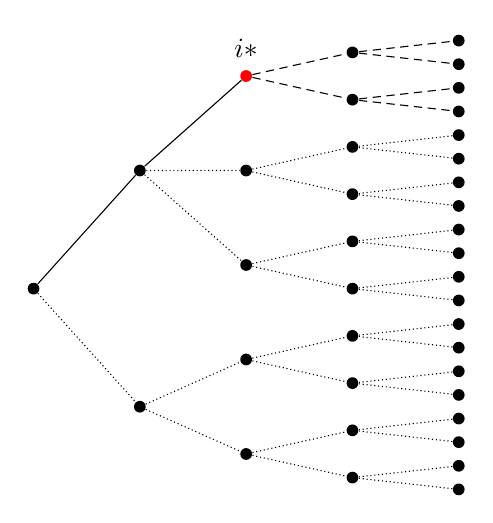
\begin{tikzpicture}
		[scale=1.5,level distance=9mm,
		every node/.style={fill=black,circle,inner sep=1.5pt},
		level 1/.style={sibling distance=10mm},
		level 2/.style={sibling distance=8mm},
		level 3/.style={sibling distance=4mm},
		level 4/.style={sibling distance=2mm},
		edge from parent/.style={draw}]
		\node {} [grow=right]
		child {node {} edge from parent[densely dotted]
			child {node {}
				child {node {}
					child {node {}}
					child {node {}}}
				child {node {}
					child {node {}}
					child {node {}}}}
			child {node {}
				child {node {}
					child {node {}}
					child {node {}}}
				child {node {}
					child {node {}}
					child {node {}}}}}
		child[missing]
		child {node {}
			child {node {} edge from parent[densely dotted]
				child {node {}
					child {node {}}
					child {node {}}}
				child {node {}
					child {node {}}
					child {node {}}}}
			child {node {} edge from parent[densely dotted]
				child {node {}
					child {node {}}
					child {node {}}}
				child {node {}
					child {node {}}
					child {node {}}}}
			child {node [style={fill=red},label=above:$ \boldsymbol{i*} $] {}
				child {node {} edge from parent[densely dashed]
					child {node {}}
					child {node {}}}
				child {node {} edge from parent[densely dashed]
					child {node {}}
					child {node {}}}}};
\end{tikzpicture}\end{figure}







\Citet{VonPrince2017a,VonPrince2019} establishes a formal trichotomy between the \textsc{actual, potential} and \textsc{counterfactual} domains by appealing to this framework. This is reproduced in (\nextx).

\pex Given a contextually defined \textsc{actual present} $( i*=\langle w*,t*\rangle )$, $ \mathcal I $ can be partitioned into three subdomains:
\a The \textsc{actual} (past/present) = $ \{i\mid i\preceq i*\} $\\
Compare this notion to the equivalent one of \textit{metaphysical alternatives to $ w $ at $ t $} introduced in Ch. \ref{bambai}: $ \{w'\mid w\approx_t w\} $.
\a The \textsc{potential} (future) = $ \{i\mid i\succ i*\} $
\a The \textsc{counterfactual} = $ \{i\mid i \text{ is unordered w/r/t } i* \} $\deftagex{trichot}\deftagpage{vP-bt}
\xe


\subsection{Semantics of modal particles}

Shown in \S\ref{desc-ii}, \textit{dhu} `\gls{fut}' occurs in sentences with future temporal reference (\getref{dhu-fut}). Relatedly, the data in (\getref{dhu-nec}) show that \textit{dhu} appears to also be compatible with other circumstantial modalities; in a deontic (a), bouletic (b) and teleological (c) context. In all these contexts, we can model \textit{dhu} as universally quantifying over a (subset of) a circumstantial modal base.

\pex \textbf{\textit{dhu} `\gls{fut}' encoding future tense with \textbf{I-} and \textbf{II}-inflections}
\a\begingl\gla barpuru goḏarr ŋarra \textbf{dhu} nhä-\textbf{ŋu}//
\glb funeral tomorrow 1s \gls{fut} see-\textbf{II}//
\glft`I'll watch the funeral tomorrow.'\trailingcitation{}\deftagex{dhu-fut}//
\endgl
\a\begingl\gla mukul \textbf{dhu} \textbf{gi} nhin-\textbf{i} raŋi-ŋur goḏarr//
\glb aunt \textbf{\gls{fut}} \gls{ipfv}.\textbf{II} sit-\textbf{II} beach-\gls{loc} tomorrow//
\glft`Aunty will be sitting on the beach tomorrow.'\trailingcitation{[AW~20190409]}//\endgl
\a\begingl\gla limurru \textbf{dhu} ḻuk-\textbf{a} maypal yalala milmitjpa//
\glb 1d.\textsc{excl} \textsc{fut} consume-\textbf{I} shellfish later evening//
\glft `We're having shellfish this evening.'\trailingcitation{[DG~20190417]}//
\endgl
\xe
\pex \textbf{\textit{dhu} `\gls{fut}' and other flavours of modal necessity}\deftagex{dhu-nec}
\a\begingl\gla Way! Nhe \textbf{dhu} gurruk-\textbf{ama} djoŋgu'!//
\glb Hey! 2s \gls{fut} carry-\textbf{I} hat//
\glft`Hey! You must wear a helmet!'\trailingcitation{[DG~20190405]}//\endgl
\a\begingl\gla djamarrkuḻi \textbf{dhu} yaka wurraŋatjarra'\textbf{y-irr}//
\glb children \gls{fut} \gls{neg} cruel.\gls{inch}-\textbf{I}//
\glft`The children mustn't be disobedient.'\trailingcitation{[AW~20190429]}//\endgl
\a\begingl\gla ŋarra \textbf{dhu} plane-dhu marrtji, bili mutika-miriw//
\glb 1s \gls{fut} plane-\gls{erg} go-\textbf{I|II} \gls{cplv} car-\gls{priv}//
\glft`I'll have to go by plane because I don't have a car.'\trailingcitation{[AW~20190429]}//\endgl
\xe


\begin{figure}[h]\centering\caption{(In)compatibility of modal particle \textit{dhu} `\gls{fut}' with temporal reference \& inflectional category.}\label{FutSchem}
	\begin{tikzpicture}[scale=.9]
		% draw horizontal line   
		\draw[<->, line width=.5mm] (0,0) -- (12,0);
		
		%draw rex
		\fill[gray!10!white] (0,0.02) rectangle (4.8,1.5);
		%	\fill[green!10!white] (2.5,0.02) rectangle (4.8,1.5);
		\fill[gray!10!white] (4.8,0.02) rectangle (6.8,1.5);
		\fill[green!10!white] (6.8,0.02) rectangle (9.5,1.5);
		\fill[orange!10!white] (9.5,0.02) rectangle (12,1.5);
		
		% draw nodes
		\draw (1.25,0) node[below=3pt] {\textbf{}} node[above=10pt] {\textsc{\textbf{*}}};
		\draw (3.675,0) node[below=3pt] {\textbf{}} node[above=10pt] {\textbf{*}};
		\draw (5,0)   node[circle,fill,label=below:$\lfloor{\sl today}$] {} node[below=3pt] {\textbf{}} node[above=3pt] {};
		\draw (7,0) node[diamond,shade,inner color=ochre,outer color=black,label=below:$\boldsymbol{t*}$] {} node[below=3pt] {\textbf{}} node[above=3pt] {\textsc{}};
		\draw (5.8,0) node[below=3pt] {\textbf{}} node[above=10pt] {\textsc{\textbf{*}}};	
%		\draw (7.5,0) node[below=3pt] {\textbf{}} node[above=10pt] {\textsc{\textbf{II}}};
		\draw (8.25,0) node[below=3pt] {\textbf{}} node[above=10pt] {\textsc{\textbf{I}}};	
		\draw (10.75,0) node[below=3pt] {\textbf{}} node[above=10pt] {\textsc{\textbf{II}}};	
		\draw (9.5,0)   node[circle,fill,label=below:${\sl today}\big)$] {} node[below=3pt] {\textbf{}} node[above=3pt] {};
		
		%		%braces
		%		\phantom{	\draw [decorate,decoration={brace,amplitude=4pt},xshift=-0pt,yshift=35pt]
		%			(0.5,0.5) -- (4.5,0.5) node [black,midway,yshift=0.35cm] 
		%			{\footnotesize metricality};
		%
		%			\draw [decorate,decoration={brace,amplitude=4pt},xshift=-0pt,yshift=40pt]
		%			(3.5,0.5) -- (9,0.5) node [black,midway,yshift=0.35cm] 
		%			{\footnotesize cyclicity};}
		
	\end{tikzpicture}
\end{figure}


On the basis of this range of usage, we might adopt the following lexical entry for \textit{dhu}, treating this particle as a modal expression and adapting the meaning of \textit{will} provided in \citet{Condoravdi2002,Condoravdi2003}. The function \textsc{best} selects the best worlds in a circumstantial modal base, according to a set $ o $ of: • speaker expectations (in the case of \textsc{future} uses), • relevant rules \& regulations (in the case of \textit{deontic} uses), • relevant wants (in the case of \textit{bouletic} uses) or • in view of achieving relevant ends (in the case of \textit{teleological} uses) \textit{etc.} We lexically specify the modal base on account of the apparent incompatibility between WD modal particles and epistemic conversational backgrounds (\citealp[e.g.][]{Peterson2010,Kratzer2012} a.o.).



\pex \deftagex{dhu-sems}$ \denote{\textit{dhu}}=\lambda o\lambda m\lambda P\lambda i:\forall b\ni i\big[b\in\underset{o}{\textsc{best}}\big(\underset{\textsc{circ}}{\cap m(i)}\big)\to\exists i'\in b[i'\succeq i\wedge \textsc{at}(P,i)]\big] $

%.\forall w'\big[w'\in\underset{o}{\textsc{best}}\big(\cap\textsc{circ}(w),t\big)\to \textsc{Inst}\big(P,w',[t,\infty)\big)\big]$\\
\textit{dhu $ P $} %, uttered in some reference index $ i $,
 asserts that -- in the best branches that contain the reference index $ (b\ni i) $ (according to some ordering source $ o $) -- the property $ P $ is instantiated in the at some index $ i' $ that is a successor to $ i $.\footnote{The relation ``\textsc{Inst}antiation'' (also given as \textsc{at}) is taken to hold between a property of events, a time, and a world when there is some event of a given type that is contained within that time: $$ \textsc{Inst}(P,w,t)=\exists e[P(e)\wedge\tau(e,w)\sqsubseteq t] $$ See also \citet{Condoravdi2003,Condoravdi2014} a.o.}\marginnote{it seems that M16,R+M18 treat the circ. mb as a presupposition: i.e. relevant modals are defined iff $ f $ is circ.}
\xe\marginnote{potentially want to say that \textsc{inst} holds at $ t* $}[-1in]


In addition to \textit{dhu}, WD deploys a number of other modal particles: \textit{balaŋ(u)} `\gls{irr}' the most frequently occurring among them. \textit{balaŋ(u)} occurs with verbal predicates categorically inflected for either \textbf{II} (shown in \getref{balaŋ-ii}) or \textbf{IV} (shown in \getref{balaŋ-iv}).

The distinction in interpretation between these two sets of data is the \textit{temporal interpretation} of the modal. In all cases \textit{balaŋ(u)} appears to trigger existential quantification over a circumstantial modal base, although whereas \textbf{II}-marking induces a future interpretation of the predicate, \textbf{IV}-marking induces a past possibility (including counterfactual) reading.

\marginnote{\textit{balaŋ} may be better glossed as just \gls{mod}, where \gls{irr} is reserved to describe verbal mood.}
\pex \textbf{\textit{balaŋ(u)} `\gls{irr}' and \textbf{II}-inflection}\deftagex{balaŋ-ii}

\a\begingl\gla ŋarra \textbf{balaŋu} (bäynha)\footnotemark dhiŋg-\textbf{uŋu} nawalulyu//
\glb 1s \textbf{\gls{irr}} (\gls{mod}) die-\textbf{II} smoke.\gls{erg}//
\glft`I could die from the smoke.'\trailingcitation{[DG~20190405]}//\endgl
\a\begingl\gla ŋarra \textbf{balaŋu} ḻuk-\textbf{i} gapu, ŋanydja monuk ŋayi gapu//
\glb 1s \textbf{\gls{irr}} consume.\textbf{II} water but saline 3s water//
\glft`I would drink some water but this water's salty.'\trailingcitation{[DG~20190405]}//\endgl
\a\begingl\gla ŋarra ŋuli ga bitjan bili warguyun ŋunhi recorder \textbf{balaŋu} bakthu-\textbf{rru}//
\glb 1s \gls{hab} \gls{ipfv}.\textbf{I} thus.\textbf{I} \gls{cplv} worry.\textbf{I} \gls{texd} recorder \textbf{\gls{irr}} break-\textbf{II}// 
\glft`I'm always worried that the recorder will/could break.'\trailingcitation{[DG~20190417]}//\endgl
\xe
\footnotetext{Here I treat \textit{bäynha} as semantically identical to \textit{balaŋ(u)}.}
\pex \textbf{\textit{balaŋ(u)} `\gls{irr}' and \textbf{IV}-inflection}\deftagex{balaŋ-iv}

\a\begingl\gla nhe \textbf{balaŋu} malkthu-\textbf{nha}//
\glb 2s \textbf{\gls{irr}} accompany-\textbf{IV}//
\glft `you should/would have gone with (him).'\trailingcitation{[DG~20190413]}//\endgl


\a\begingl\gla ŋarra gana guyaŋa-na waṯuy \textbf{balaŋu} ḻuka-\textbf{nha} chocolate//
\glb 1s \gls{ipfv}.\textbf{III} think-\textbf{III} dog.\gls{erg} \textbf{\gls{irr}} eat-\textbf{IV} chocolate//
\glft`I'd thought the dog might/would eat the chocolate.'\trailingcitation{[DG~20190413]}//\endgl

\a\begingl\gla ŋarra-nha \textbf{balaŋu} ḻuku walala mitthu-\textbf{na}... yurru ŋarra manymak-thirri//
\glb 1s-\gls{acc} \textbf{\gls{irr}} foot 3p cut-\textbf{IV} but 1s good-\gls{inch}.\textbf{I}//
\glft`They would have amputated my foot, but I got better.'\trailingcitation{[DG~20190417]}\deftaglabel{ḻuku}//\endgl
\xe
\marginnote{I actually don't currently have any way of specifying that \textit{dhu} is necessarily assumes pres-persp \& future-orientn unlike \textit{balaŋ}.}

\begin{figure}[h]\centering\caption{Compatibility of modal particle \textit{balaŋ} `\gls{irr}' with temporal reference \& inflectional category.}\label{BalSchem}
	\begin{tikzpicture}[scale=.9]
		% draw horizontal line   
		\draw[<->, line width=.5mm] (0,0) -- (12,0);
		
		%draw rex
		\fill[violet!10!white] (0,0.02) rectangle (6.8,1.5);
		%	\fill[green!10!white] (2.5,0.02) rectangle (4.8,1.5);
%		\fill[gray!10!white] (4.8,0.02) rectangle (6.8,1.5);
%		\fill[green!10!white] (6.8,0.02) rectangle (9.5,1.5);
		\fill[orange!10!white] (6.8,0.02) rectangle (12,1.5);
		
		% draw nodes
%		\draw (1.25,0) node[below=3pt] {\textbf{}} node[above=10pt] {\textsc{\textbf{*}}};
		\draw (3.675,0) node[below=3pt] {\textbf{}} node[above=10pt] {\textbf{IV}};
		\draw (5,0)   node[circle,fill,label=below:$\lfloor{\sl today}$] {} node[below=3pt] {\textbf{}} node[above=3pt] {};
		\draw (7,0) node[diamond,shade,inner color=ochre,outer color=black,label=below:$\boldsymbol{t*}$] {} node[below=3pt] {\textbf{}} node[above=3pt] {\textsc{}};
%		\draw (5.8,0) node[below=3pt] {\textbf{}} node[above=10pt] {\textsc{\textbf{*}}};	
		%		\draw (7.5,0) node[below=3pt] {\textbf{}} node[above=10pt] {\textsc{\textbf{II}}};
%		\draw (8.25,0) node[below=3pt] {\textbf{}} node[above=10pt] {\textsc{\textbf{I}}};	
		\draw (9.5,0) node[below=3pt] {\textbf{}} node[above=10pt] {\textsc{\textbf{II}}};	
		\draw (9.5,0)   node[circle,fill,label=below:${\sl today}\big)$] {} node[below=3pt] {\textbf{}} node[above=3pt] {};
		
		
	\end{tikzpicture}
\end{figure}


On the basis of these data then, we propose a lexical entry for \textit{balaŋ(u)} as in (\getref{balaŋ-sems}) below. \textit{balaŋ(u)} is taken to differ from \textit{dhu} in terms of the ``force'' of the modal quantification it realises, in addition to its lability with respect to instantiation time.

\pex\deftagex{balaŋ-sems}
$ \denote{\textit{balaŋ(u)}} = \lambda o\lambda m\lambda P\lambda i.\exists b\ni i'\big[b\in\underset{o}{\textsc{best}}\big(\underset{\textsc{circ}}{\cap m(i)}\big)\wedge\exists i'\succeq i\wedge \textsc{at}\big(P,i)\big]$\\
Defined iff the modal base $ m $ is circumstantial, \textit{balaŋ(u)} $ P $ is true iff one of the best (according to $ o $) branches $ b $ that contains the reference index.......
%\lambda o\lambda P\lambda w\lambda t.\exists w'\big[w'\in\underset{o}{\textsc{best}}\big(\cap\textsc{circ}(w),t\big)\wedge \textsc{Inst}\big(P,w',(t,\infty)\big)\big] $
\xe
\marginnote{There's this right edge thing in the instantiation interval acc. C02 which apparently is constrained by past tense, i'm not sure how or whether this needs representing. there's also the nonactuality implicature that comes out at the end of the paper which maybe could do the nec. work?}


The distinction between the temporal interpretations in \textbf{II}- and \textbf{IV}-inflected clauses then in effect reflects the distinction drawn by \citet{Condoravdi2002} between \textit{present} and \textit{past} \textsc{temporal perspective} respectively. For \citet[62\textit{ff}]{Condoravdi2002}, temporal persepctive is the time at which some modal claim is calculated. A counterfactual predication like (\getfullref{balaŋ-iv.ḻuku}), for example, communicates that `we are now located in a world whose past included the (unactualized) possibility of a foot amputation. The contribution of \textit{balaŋ} is spelled out in (\nextx).

\ex  
\begingl\glpreamble\textit{balaŋu} on a counterfactual reading (past temporal perspective contributed by \textbf{IV})//
\gla ŋarra-nha \textbf{balaŋu} ḻuku walala mitthu-\textbf{na}//
\glb 1s-\gls{acc} \textbf{\gls{irr}} foot 3p cut-\textbf{IV}//
\glft`They would have amputated my foot.'\trailingcitation{[DG~20190417]}//\endgl\\

\denote[c]{(\getfullref{balaŋ-iv.ḻuku})} iff $ \exists i',i''\big[i'\prec i_c\wedge\exists b\ni i'[b\in\textsc{mb}(i')\wedge i''\succ i'\wedge\denote[i'']{(\getfullref{balaŋ-iv.ḻuku})})]\big] $\\
%$ \exists w',t',t''\big[t'\prec t\wedge\in\textsc{mb}(w,t')\wedge t'\prec t''\wedge\denote[w',t'']{(\getfullref{balaŋ-iv.ḻuku})})\big] $\\
In words: at an evaluation index, the proposition is true if, in the past of that index, there was some future index at which the proposition is true.%\trailingcitation{[adapted from \citealp[62-3]{Condoravdi2002}]}
\xe

\subsection{Semantics of the ``\textsc{nonrealised}'' inflections}\label{mood-lit}


Various authors in the functional-typological tradition have identified a semantic category in \textsc{reality status}, (perhaps) to be distinguished from \textsc{mood} and (perhaps also from) \textsc{modality} (\citealp[see][]{Bowern1998,Elliott2000,Roberts1990a,Michael2014,McGregor2006,Mithun1995,Chafe1995}.) For these authors, significant utility is to be found in drawing a broad dichotomy between \textsc{realis} and \textsc{irrealis}: that is, propositions can be taken as either a description of eventualities that correspond with observed/observable reality versus a description of a hypothetical, imagined, non-actualised eventuality. Consequently, for its defenders, \textsc{irrealis} can be conceived of as whatever semantical concept might be taken to collect: future, modalised and conditional predications and imperatives, in addition (for some languages) to negative and habitual predications and interrogatives \citep[see also][]{Palmer2001,Givon1994,Plungian2005}.\footnote{Conversely, \citet{Cristofaro2012} explicitly takes issue with the inference that linguists have made that the notion of irreality ``plays some role in [the use of irrealis-denoting forms]'' (132), which she attributes to a broader methodological issue in the discipline --- \textit{viz.} that description of observed grammatical patterns should be kept distinct from the formulation of explana- tory generalizations about these patterns, including generalizations about particular grammatical categories'' (145).} 

Conversely, the concept of \textsc{reality status} and the \textit{realis/irrealis} distinction has also been roundly criticised by a number of authors, predominantly due the fact that few languages appear to grammaticalise the realis/irrealis contrast as a ``binary morphological distinction'' as well as the apparent heterogeneity of these categories cross-linguistically. That is, the semantic domain of an \textsc{irrealis} marker on the basis of the analysis of one language tends tends to include and exclude parts of the semantic domain of others (\citealp[see][238]{Bybee1994}, \citealp[\textit{apud}][158\textit{ff}]{Foley1986}. \citealp[See also, \textit{e.g.},][]{Bybee1998,Portner2018a,Haan2012}.) Of course, the actual semantic contribution of any given class of marker can vary radically across languages, whence the difficulty in providing a unified semantics for, \textit{e.g.}, the Romance subjunctive.

On the basis of cross-linguistic data, \citet[138\textit{ff}]{Cristofaro2012} argues that there languages crucially tend to draw a distinction between `as-yet unrealized' and `non-realized (in the past)' -- \textit{i.e.}, these domains are grammaticalized separately. She deploys this observation to argue against an empirical basis for a unified \textsc{irrealis} category --- suggesting that the ``multifunctionality'' for a given form ought to be attributable to ``contextual inference'' or ``generalization'' rather than furnishing evidence of the semantic import a dichotomous reality status category. Relatedly, \citet[467]{Portner2012} make a parallel observation regarding a potential necessity to ``invoke  grammaticalization'' in their analysis of subjunctive-selecting predicates in Romance --- suggesting that in at least some cases (\textit{sc.} for some predicates) the \textsc{indicative/subjunctive}  distinction is inert.
	

Nevertheless, the co-occurrence constraints between the ``irrealis-aligned inflections'' \textbf{II} and \textbf{IV} and modal expressions described above (\textit{e.g.}, \textit{dhu }and\textit{ balaŋ(u)}) suggest a semantic treatment of these inflections that aligns with current analyses of verbal mood --- those where the ``subjunctive'' paradigms of various European languages are taken to be ``obligatory and redundant'' --- dependent on a range of irrealis-aligned (modal) operators, predominantly propositional attitudes \citep{Palmer2001}.\footnote{\citet[238]{Chung} explicitly suggest an equivalence between \textsc{realis} and the \textsc{indicative}. See also \citealt{Matthewson2010} on the St̓át̓imcets ``subjunctive'' and for a discussion (following \citealt{Palmer2001}) of a proposed distinction between \textsc{subjunctive} and \textsc{irrealis} as grammatical categories. In large part, authors seem to treat the distinction as stemming from the fact that \textsc{subjunctive} morphology is often restricted to syntactically subordinate clauses (i.e. the complement of particular verbal predicates) --- likely in addition to established descriptive traditions for European languages (\citealp[see also][169\textit{ff}]{Mauri2016}, \textit{cf. }\citet[13, fn 9]{Matthewson2010} who takes issue with this criterion).} \citet[§ 2.2]{Portner2018a} identifies two broad sets of intuitions about the semantics of verbal mood (predominantly on the basis of the \textsc{indicative-subjunctive} contrast in a number of European languages) which have driven analytic work: analyses that hinge on the semantics of \textbf{comparison} versus \textbf{truth in a designated set of worlds}. Comparison-based approaches claim that, iff a given predicate involves a non-empty ordering source (\textit{i.e.}, involves comparison \& relative rankings of possible worlds), it will select for a subjunctive complement. Truth-based approaches generally claim that the function  of the \textsc{indicative} is to assert the truth of a given clause in some set of worlds --- in effect, the \textit{realis} domain.\footnote{\citet{Portner2018a} takes comparison-based analyses to be exemplified in \citealt{Portner2012,Anand2013,Giorgi1997,Villalta2008} and truth-based analyses to include \citealt{Giannakidou2011,Farkas1992,Farkas2003,Huntley1984,Quer2001,Portner1997}. Although as noted here, for him the ``current state of the art in mood semantics'' appears to unite/``treat as correct'' both of these observations.} On the basis of this generalisation, \citeauthor{Gian2016} (2016), \citealp{Giannakidou2020}) a.o. take the subjunctive to indicate ``nonveridicality'' with respect to a proposition --- that is, it indicates that there exists at least one world in a given set of worlds in which that proposition is not true (schematised in \nextx.)

\pex $ M $ is \textbf{nonveridical} w/r/t $ p $ iff\\
$ \exists w' [w'\in M\wedge w'\in\neg p]$\trailingcitation{\citep[see][190]{Gian2016}}
\xe

 \citet[71]{Portner2018a} argues, these two intuitions ought to be unifiable (the \textit{``proto-standard theory of mood''}, \citealp[see also][]{Portner2018,Portner2012}) given that ordering semantic approaches effectively designate a ``most relevant'' set of worlds in the modal base which can be taken to be the set of worlds for which truth is being asserted in indicative-marked clauses. Drawing inspiration from a number of these approaches, we can posit a semantics that captures intuitions about the ``irrealis''-alignment of the \textbf{II} and \textbf{IV} inflections.


In effect, I take \textbf{II} and \textbf{IV} to realise the temporal contribution of \textbf{I} and \textbf{III} respectively, while also enforcing a presupposition of \textbf{nonveridicality} with respect to the eventuality introduced by given predicate. This hypothesis is summarised in (\getref{irr-hyp}) and spelled out in the section below.

\pex\textbf{Licensing conditions for \gls{irr}}\deftagex{irr-hyp}
\a \textbf{II} and \textbf{IV} are the irrealis counterparts of the temporal inflections \textbf{I} and \textbf{III} (that is, they impose the same set of temporal constraints on the instantiation of their prejacent.
\a They additionally presuppose \textbf{nonveridicality} with respect to the modal frame of the local clause\footnote{See also the ``locality of binding'' principle in  \citealp[201]{Percus2000}, 	\citealp[99]{Hacquard2010}.}
\xe



\subsubsection{Subjunctivity}


The discussion above draws on the literature on \textsc{verbal mood}, an enterprise which attempts to capture intuitions about the meaning contrasts between the \textsc{indicative} and \textsc{subjunctive} categories of (almost exclusively)\footnote{As mentioned \citet{Matthewson2010} describes mood morphology in St̓át̓imcets th.at she argues is a realisation of a \gls{sbjv} category.} European languages. In his comparison of \textsc{irrealis} and \textsc{subjunctive} as putative grammatical categories, \citet[186]{Palmer2001} in part attributes these distinct metalinguistic conventions to different ``different traditions'', but also notes that an apparent difference between the categories; namely that, ``[\gls{sbjv}]is generally redundant only in subordinate clauses, where the subordinating verb clearly indicates the notional feature.'' Conversely, \gls{irr} is frequently found in matrix clauses, co-occurring with other modal expressions.

\pex\a\begingl\glpreamble French \textsc{subjunctive}//
\gla Il faut qu'[il se \textbf{taise}]//
\glb 3s be.necessary.\gls{indic} \gls{comp}\textdblhyphen{3s} \gls{refl} be.quiet.\textbf{\gls{sbjv}}//
\glft`It's necessary that he be quiet.'//\endgl
\a\begingl\glpreamble Caddo \textsc{irrealis}//
\gla kas-\textbf{sa}-náyʔaw//
\glb \textsc{oblig}-3\textsc{ag}.\textbf{\gls{irr}}-sing//
\glft`He should/is obliged to sing.'\trailingcitation{\citep[356]{Chafe1995}}//\endgl
\xe


Crucially, WD inflections are \textbf{not sensitive to} embedding predicates. Canonical subjunctive-licensing predicates like `want' do not in themselves trigger an \gls{irr}-aligned inflection.

\pex Desiderative embedding predicate doesn't license mood shift in WD\trailingcitation{\citep[23]{Wilkinson}}
\a\begingl\gla walal ga djälthi-rr walala-ny dhu \textbf{gäma} hunting-lil wämut-thu//
\glb 3p \gls{ipfv}.\I{} want-\I{} 3p-\gls{prom} \gls{fut} take.\I{} \textit{hunting}-\gls{all} \gls{malk}-\gls{erg}//
\glft`They want that Wämut take them hunting.'//\endgl
\a\begingl\gla ŋuriki waṯu-w ŋarra ga djälthi-rr ŋayi dhu ḏarrkthu-\textbf{n} nhuna-ny//
\glb \gls{texd}.\gls{dat} dog-\gls{dat} 1s \gls{ipfv}.\I{} want.\I{} 3s \gls{fut} bite-\I{} 2s.\gls{acc}.\gls{prom}//
\glft`I want of that dog that it bite you.'//\endgl\marginnote{a-b actually don't demonstrate this because they're embedding dhu-sentences anyway (which is in itself notable given the future orient of want predicates x-linguistically)}
\a\begingl\glpreamble From Djr bible Mäk 6:19.//
\gla Bala ŋayiny ŋunhi miyalktja ŋoy-dhärra-na-n nhanŋu Djon-gu-ny, ga djälthinany ŋayi gan bunharawnha nhanŋu murrkay'kunharawnha yan, yurr bäyŋu.//
\glb \gls{mvtawy} 3s.\gls{prom} \gls{texd} woman.\gls{prom} soul-stand-\III-\gls{seq} 3s.\gls{dat} John-\gls{dat}-\gls{prom} and want-\gls{inch}-\III 3s \gls{ipfv}.\III kill-\IV-\gls{dat}-\gls{seq} 3s.\gls{dat} hard-\gls{caus}.\IV.\gls{dat}.\gls{seq} \gls{emph} but \gls{negq}//
\glft`So that woman was upset with John and she was desirous of his violent death.'//\endgl
\xe


Similarly surprising, as with embedding predicates the epistemic adverb \textit{mak(u)} is also completely invisible to the inflectional paradigm.

\pex
\begingl\glpreamble{Epistemic \textit{mak(u)} doesn't license mood shift in WD}//
\gla maku ga nhina raŋiŋura maku bäyŋu. Yaka marŋgi.//
\glb \gls{epist} \gls{ipfv}.\I{} sit.\I{} beach-\gls{loc} \gls{epist} \gls{neg} \gls{neg} know//
\glft`Maybe she's at the beach, maybe not. Dunno.'\trailingcitation{[DB~20191416]}//\endgl
\xe

Given that the mood-shift in WD inflections appears to be triggered within the clause by root modals (to the exclusion of subordinating attitude predicates and epistemic modal expressions), diverging from the canonical distribution of subjunctive morphology in Europoean languages, we have reason \citep[following][]{Palmer2001} to treat the mood category inflected on WD verbs as \textsc{irrealis}.

\subsubsection{Modelling assumptions}

I assume that verbs in WD denote properties of events $ \langle \varepsilon,st\rangle $. These are bound by aspectual operators, which existentially bind the event variable and map them to temporal properties $ \langle\imath,st\rangle $  (a standard assumption, \citealp[see][]{Kratzer1998}). Denotations for aspect operators, including the inflecting auxiliary \textit{GA} `\gls{ipfv}' and a covert \gls{pfv} operator are given below in (\nextx).\footnote{Of course there are considerably more sophisticated treatments of aspect in the semantics literature (\citealp[e.g.,][]{Deo2009a,Dowty1979} a.o.) Nothing in the forthcoming analysis is reliant on the one provided here, which is similar to that described in \citet{Taylor1977}.}

\pex Denotations for WD aspectual operators
\a$ \denote{\textit{ GA }}= \lambda P_{\langle\varepsilon,st\rangle}\lambda i.
%\exists i'\big[i'\sqsupseteq i \wedge
\exists e[P(e)\wedge \tau(e)\sqsupset i]$
\a$ \denote{\textsc{pfv}}= \lambda P_{\langle\varepsilon,st\rangle}\lambda i.
%\exists i'\big[i'\sqsupseteq i \wedge
\exists e[P(e)\wedge \tau(e)\sqsubset i]$

\xe
WD aspect morphology existentially binds the event variable in a property of events, mapping it to a property of indices. \textit{GA} `\gls{ipfv}' asserts that the reference index $ (i) $ is contained within the event's runtime $ \tau(e) $, $ \varnothing $ `\gls{pfv}' asserts that $ \tau(e) $ is contained within $ i $.

The WD (root) modal expressions (\textit{e.g.}, \textit{dhu} and \textit{balaŋu}, described in \getref{dhu-sems} \& \getref{balaŋ-sems} above) take a predicate $ P $ in their scope and determine the subset of relevant worlds (indices) in which $ P $ holds. That is, they express a restriction over the modal base, in effect encoding \textbf{objective nonveridicality}.




Additionally, The LF of a simple (unembedded) clause is taken to be headed by a silent \textsc{assert} operator (similar assumptions made in \citealt{Hacquard2010,AlonsoBenito2015,Kaufmann2005}) which takes an inflected proposition as its sister.\footnote{A similar strategy (in the spirit of update semantics) is adopted in \citealt[570]{Krifka2016}, where \textsc{assert} is taken to perform an operation on a common ground. See also references in \citealt[102]{Hacquard2010}.} This approach effectively formalises (some) ideas about the illocutionary force and sets of norms that apply to assertoric speech acts (\citealp[e.g.][]{Williamson1996,Brandom1983} a.o.) by postulating a covert doxastic modal which is anchored by the actual world $ i* $. $ \sim_\alpha $ is a doxastic accessibility relation anchored to some individual $\cap\alpha $.

\pex \textbf{An assertability relation}\\
$ \denote{\textsc{assert}}_{\langle s,\langle s,t\rangle\rangle}
=\lambda i.\cap\sim_\alpha i $

%$\denote{\textsc{assert}} = \lambda p\lambda w.\forall w'[w'\in\mathcal B_{\text{Spkr}_c} (w)\to p(w')]$\\
\textsc{\textsc{Assert}} is an accessibility relation that, given a speech index $ i $ returns all the propositions that are believed/``assertable'' by a given judge $ \alpha $ at that index.
%$ c $ iff $ p $ holds in all of the speaker's belief worlds.
\xe%\marginnote{\cite[238,250ff]{Kaufmann2005} is more %insightful: will probably try to model this on his $ \sim $ instead}

The force of this model can additionally be weakened by epistemic possibility adverb \textit{mak(u)}. Given its apparent variable modal force, \textit{maku} takes an accessibility relation (\textit{e.g.}, \textsc{assert}) as its sister and returns a subset of the modal base it picks out.  Following \citealt{Matthewson2010,Rullmann2008} a.o., force-variable modality is modelled as universal quantification over a a (contextually-determined) subset of the modal base (as determined by a ``contextually given'' choice function $ f_c $.) Modal strength, then, is proportional to the proportion of the modal base that is understood to be quantified over.

%, analysed here as a propositional modifier \citep[\textit{e.g.},][]{Hacquard2010}. Like \textsc{assert}, this modal expression is lexically restricted to quantify over an epistemic modal base (\citealp[cf.][]{Matthewson2016} a.o.). %:\footnote{Diverging from \citet[997\textit{ff}]{Yalcin2007}, \citealt[106]{Hacquard2010} takes epistemic modals to be merged underneath the \textsc{assert} operator in order to maintain a unified lexical entry for root and epistemic modals --- as a result, in view of the fact that it retrieves an identical quantificational domain, the contribution of \textsc{assert} scoping over an epistemic modal is vacuous. Given that \textit{mak(u)} admits only only of epistemic readings}

\pex \textbf{Epistemic possibility}
\a$\denote[]{\textit{mak(u)}}_{\langle\langle s,\langle s,t\rangle,\langle s,\langle s,t\rangle\rangle} = \lambda r_{\langle s,\langle s,t\rangle\rangle}.f_c(r)$
\a$ \denote{\textit{maku}}(\denote{\textsc{assert}}) =\lambda i.f_c(\cap\sim_\alpha i)$
%\lambda p\lambda w.\exists w'[w'\in\mathcal B_{\text{Spkr}_c} (w)\wedge p(w')]$\\




\xe


With these assumptions in place, we can propose lexical entries for the verbal inflections.


\subsubsection{Nonveridicality as presupposition}

The WD inflections, then, all denote partial functions. 
They provide temporal information about a given proposition by existentially binding the time variable (compare \getref{disjunct}, replicated in \nextx).

Additionally, the nonveridicality constraint is modelled as a presupposition that the truth of the inflected sentence does not follow from (that is, it is unsettled) in the evaluation context: in a simple/matrix clause, the evaluation context is to be understood to be anchored to the speakers belief state in the actual world.




\pex\a$\denote{\textbf{\II}}=\lambda P_{\langle s,t\rangle}\lambda i_s:\exists i'\in\cap\approx_i\wedge\neg P(i').P(i)$

\II~presupposes that there is some metaphysical alternative to the reference index $ i $ at which $ P $ doesn't hold.\\It asserts that $ P $ holds at $ i $.

\a$ \denote{\IV}=\lambda P_{\langle s,t\rangle}\lambda i_s:\exists i'\in\cap\approx_i\wedge\neg P(i')\wedge\exists j\underset{\text{final}}{\sqsubseteq} i.\textsc{nfInst}(P,i,j)$

\IV~presupposes that there is some metaphysical alternative to the reference index $ i $  which $ P $ doesn't hold and asserts that $ P $ is instantiated at some non-final subinterval of $ i $.

\xe\marginnote{This actually doesn't get the temporal stuff to come out right, it seems to require stuff to be instantiated at speech time. Need to add another index (see cyclic tense stuff.)}





%\pex
%\a$\llbracket\textbf{II}\rrbracket^{c}=\lambda p_{\langle\imath,\langle s,t\rangle\rangle}\lambda\mathcal{A}_{\langle s,t\rangle}\begin{matrix*}[l]:\exists w'[w'\in\mathcal{A}\wedge w'\notin p]\\.\exists i\begin{cases}i\not\prec today\leftrightarrow i\succeq i*&.\,P(w)(i)\textsc{[nonpast]}\\
%	i\prec today \leftrightarrow \mu(i,i*)<s_c&.\,P(w)(i)\textsc{[recent past]}
%\end{cases}\end{matrix*}$
%
%\textbf{II} presupposes that $ p $ doesn't follow from the set of worlds $ \mathcal A $.
%It asserts that $ P $ holds at $ i $ where:\\
%\textbf{\textsc{either}} the reference time $ i$ doesn't precede speech time $ i*$,\\ \textbf{\textsc{or}} if $ i $ \textsc{precedes}  $ today $, then the temporal distance by which $ i $ precedes $ i* $ is \textit{\textbf{below} some contextually provided standard} $ s_c $
%
%\a$\llbracket\textbf{IV}\rrbracket^{c}=\lambda p_{\langle\imath,\langle s,t\rangle\rangle}\lambda\mathcal{A}_{\langle s,t\rangle}
%\begin{matrix*}[l]
%:\exists w'[w'\in\mathcal{A}\wedge w'\notin p]\\.\exists i
%
%\begin{cases}i\sqsubseteq today\leftrightarrow i\prec i*&.\,P(w)(i)\qquad\textsc{[today past]}\\
%	i\prec today \leftrightarrow\mu(i,i*)>s_c&.\,P(w)(i)\qquad\textsc{[remote past]}
%\end{cases}\end{matrix*}$
%
%\textbf{IV} presupposes that $ p $ doesn't follow from the set of worlds $ \mathcal A $.
%\textbf{\textsc{either}} the reference time $ i $ falls within $ today $, in which case it precedes speechtime $ i* $,\\ \textbf{\textsc{or}} if $ i $ \textsc{precedes} $ today $, the temporal distance by which $ i $ precedes $ i* $ is \textit{\textbf{above} some contextually provided standard} $ s_c $
%\xe

\hrule\hrule\vspace*{.1em}
\small
%As discussed above, in a matrix clause, a proposition is assertable  (!!!!!!!!!!!!) This doesn't work.
\begin{framed}Effectively here are the concerns:
\begin{itemize}
	\item circumstantial modals \textit{dhu, balaŋ} quantify over circ conv bkgd. \textit{dhu} is future oriented. \textit{balaŋ} is force-variable.
	\item negation can be taken to quantify over compatible worlds. 
	\item these operators need to license the irrealis.
	\begin{itemize}
\item 	Confusingly, cyclic tense is neutralised under \textit{balaŋ}. To summarise:
\item \textit{dhu} occurs with \II{} (except SDF-\I)
\item \textit{balaŋ} occurs with \II{} with nonpast persp or \IV{} with past persp
\item \textit{bäyŋu} (\textsc{neg}) occurs with \IV{} when negating a \III-past or \II{} when negating a \I-past (except SDF-\I)
	\end{itemize}
	\item the intuition is that they are nonveridical in some objective way.
	\item epistemic modals (\textit{mak(u)}) \textbf{do not} license the irrealis.
	\item propositional attitudes \textbf{do not} in themselves license the irrealis.
	\item the immediate/today future with \textbf{\textit{dhu}} \textbf{does not} license the irrealis, (including under negation) the intuition is because these future predications are assertable..

\end{itemize}
\textbf{\textit{Conditionals: not sure where these are from}}

\pex~\a\begingl\gla \rightcomment{\textcolor{violet}{\textbf{[\textsc{sbjv}]}}}\textbf{wäniya} ŋay ŋunbalaya bulu, ŋayi \textbf{guyupiya}//
\glb go.IV 3s that~way again 3s die.IV//
\glft`If he had gone that way, he would've died'//\endgl
\a \begingl\gla \rightcomment{\textcolor{ochre}{\textbf{[\textsc{cond}]}}}\textbf{wäni} ŋay ŋunbalaya bulu, ŋayi \textbf{guyupi}//
\glb go.II{} 3s that~way again 3s die.II//
\glft`If he goes that way, he'll die'//\endgl\xe
%\hrule\hrule\vspace*{.1em}
\normalsize\end{framed}




	\iffalse
		The entries i had in the FoDS talk (definitely don't get it right):
		
		
		\textbf{II} as modal-for-the-present
		
		
		$$\llbracket \textbf{II}(\varphi)\rrbracket^{w,t*,\textbf{\textsc{mb}}}\leftrightarrow\forall w^\prime\in \textsc{\textbf{mb}}(w,t*)[t*\preceq t^\prime\wedge\varphi(w^\prime,t^\prime)] $$
		\textit{$ \varphi $ holds at or after speech time in all worlds that are \textbf{mb-}accessible from $ w $}
		
		\textbf{IV} as modal-for-the-past
		
		
		$$\llbracket\textbf{IV}(\varphi)\rrbracket^{w,t*,\textbf{\textsc{mb}}}\leftrightarrow\forall w^\prime\in \textsc{\textbf{mb}}(w,t*)[t*\succ t^\prime\wedge\varphi(w^\prime,t^\prime)] $$
		\textit{$ \varphi $ holds before speech time in all worlds that are \textbf{mb-}accessible from $ w $}
	\fi

\subsubsection{The proposal in action}

\pex\begingl\gla maku ŋarra dhu gi nhäŋu mukulnha//
\glb \gls{epist} 1s \gls{fut} \gls{ipfv}.\II{} see.\II{} aunt.\gls{acc}//
\glft `Maybe I'll be seeing aunty'//\endgl\


{\small$$ \pi:\exists i'\in\cap\approx_{i*}\wedge\neg\forall b\ni i'\Big[b\in\underset{o}{\textsc{best}}\big(\cap\textsc{circ}(i)\big)\to\exists i''\in b\big[i''\succeq i'\wedge\exists e[\textsc{see}(e)\wedge\tau(e)\sqsupset i'']\big]\Big] $$}
Presupposes that at some metaphysical alternative to $ i* $, \textit{ŋarra dhu \textsc{nhä-} mukulnha} `I'll be seeing my aunt' doesn't hold.
$$ f_c(\cap\sim_{Spkr}i*)\vDash\forall b\ni i*\Big[b\in\underset{o}{\textsc{best}}\big(\cap\textsc{circ}(i)\big)\to\exists i'\in b\big[i'\succeq i*\wedge\exists e[\textsc{see}(e)\wedge\tau(e)\sqsupset i']\big]\Big] $$
Some subset (as defined by $ f_c $) of the speaker's doxastic alternatives at the speech index $ i* $ verify the (modal) claim: `For all of the best branches (according to $ m,o $) that pass through $ i* $, there is some successor index $ i' $ which is contained by the run time of an event of my seeing my aunt.

\xe\marginnote{\textbf{Infl} maybe needs to introduce variable that wants an acc. relation in order to introduce the assertability stuff in the C-layer. Kaufmann does this with Ø much lower down in the derivation.}[-1in]
\begin{tikzpicture}
	\tikzset{level 1/.style={level distance=60pt,sibling distance=130pt}}
	\tikzset{level 2/.style={level distance=60pt,sibling distance=130pt}}
	\tikzset{level 3/.style={level distance=60pt,sibling distance=130pt}}
	\tikzset{level 4/.style={level distance=60pt,sibling distance=130pt}}
	\tikzset{level 5/.style={level distance=60pt,sibling distance=90pt}}
	\tikzset{every tree node/.style={align=center}}
	\node [font=\bfseries] (cp) {CP}
	child[xshift=.5cm,yshift=1cm] {node (speccp) {$ \boldsymbol{i*} $} edge from parent[]}
	child[font=\bfseries] {node (cbar) {C{$^\prime$}}
		child[yshift=.5cm,sibling distance=145pt] {node (chead) {$\lambda i.f_c(\cap\sim_\alpha i) $} %assert node
			child[level distance=30pt,sibling distance=65pt,font=\bfseries] {node (assert) {\textsc{assert}}}
			child[level distance=30pt,sibling distance=65pt,font=\bfseries] {node (maku) {\textit{maku}}}} %maku node
		child[yshift=-.5cm,text depth=3ex,font=\bfseries] {node (ip) {IP}
			child[xshift=-1cm,font=\bfseries] {node (infl) {Infl}}
			child[yshift=-1cm,text depth=4ex,font=\bfseries] {node (modp) {ModP$ _{\langle s,t\rangle} $}
				child[xshift=-1cm,text depth=3ex,font=\bfseries] {node (dhu) {\textit{dhu}}}
				child[yshift=-1cm,text depth=3ex,font=\bfseries] {node (aspp) {AspP$ _{\langle s,t \rangle} $}
					child[text depth=3ex,font=\bfseries] {node (ipfv) {\textsc{ipfv}$_{\langle\langle\varepsilon,t\rangle,\langle s,t\rangle\rangle}$}}
					child[text depth=3ex,font=\bfseries] {node (vp) {VP}
	}}}}};
	\node at ([xshift=0cm,yshift=-.5cm]assert) [text width=1.75cm] {
		$ \lambda i.\cap\sim_\alpha i $
	};
	\node at ([xshift=0cm,yshift=-.5cm]maku) [text width=2cm] {
		$ \lambda r.f_c(r) $
	};
	\node at ([xshift=2cm,yshift=-.2cm]ip) [text width=9cm] {
		$ \lambda i:\exists i'\in\cap\approx_i\wedge\neg\denote{\textbf{ModP}}(i').\denote{\textbf{ModP}}(i)$%%%ModPnode
	};
	\node at ([xshift=0cm,yshift=-.2cm]infl) [text width=7cm] {
		$ \lambda P\lambda i:\exists i{^\prime}[i{^\prime}\in\cap\approx_{i}\wedge\neg P(i{^\prime})\big].P(i) $
	};
	\node at ([xshift=0cm,yshift=-.2cm]modp) [text width=12cm] {
		$\lambda i.\forall b\ni i[b\in\textsc{best}(\cap m(i))\to\exists i{^\prime}\in b[i{^\prime}\succeq i\wedge\exists e[\textsc{see}(e)\wedge\tau(e)\sqsupset i{^\prime}]]]$
	};
	\node at ([xshift=-.7cm,yshift=-.2cm]dhu) [text width=11cm] {
		$ \lambda P_{\langle s,t\rangle}\lambda i_s.\forall b\ni i[b\in\textsc{best}(\cap m(i))\to\exists i{^\prime}\in b[i{^\prime}\succeq i\wedge\textsc{at}(P,i{^\prime})]] $
	};
	\node at ([xshift=0cm,yshift=-.2cm]aspp) [text width=4.5cm] {
		$\lambda i.\exists e[\textsc{see}(e)\wedge\tau(e)\sqsupset i] $
	};
	\node at ([xshift=-.25cm,yshift=-.2cm]ipfv) [text width=3.95cm] {
		$ \lambda P^\epsilon\lambda i[P(e)\wedge\tau(e)\sqsupset i] $
	};
	\node at ([xshift=0cm,yshift=-.2cm]vp) [text width=1.5cm] {
		$ \lambda e.\textsc{see}(e) $
	};
\end{tikzpicture}


%\begin{tikzpicture}[scale=.7,every node/.style={align=center},level distance=40pt]\automath
%\Tree [.CP \edge[dashed];  i* [.C' [.{$ \cap f_c(\cap\sim_\alpha i*) $} {\textsc{assert}\\$ \lambda i.\sim_\alpha i $ } {\textit{maku}\\$ \lambda r.\cap f_c(r) $} ] [.{IP\\$ \lambda R:\exists b[b\in\cap\approx_i \wedge i\notin b ].$} {Infl\\$ \lambda P\lambda i:\exists i'[i'\in\cap\approx_{i}\wedge\neg P(i')\big]$} [.{ModP_{\langle s,t\rangle}\\$\lambda i.\forall b\ni i[b\in\textsc{best}(\cap m(i))\to\exists i'\in b[i'\succeq i\wedge\exists e[\textsc{see}(e)\wedge\tau(e)\sqsupset i']]]$} {\textit{dhu}\\$ \lambda P_{\langle s,t\rangle}\lambda i_s.\forall b\ni i[b\in\textsc{best}(\cap m(i))\to\exists i'\in b[i'\succeq i\wedge\textsc{at}(P,i')]] $} [.{AspP_{\langle s,t \rangle}\\$\lambda i.\exists e[\textsc{see}(e)\wedge\tau(e)\sqsupset i] $} {\textsc{ipfv}_{\langle\langle\varepsilon,t\rangle,\langle s,t\rangle\rangle}\\$ \lambda P^\epsilon\lambda i[P(e)\wedge\tau(e)\sqsupset i] $} [.{VP_{\langle\varepsilon,t\rangle}\\$ \lambda e.\textsc{see}(e) $} ] ] ] ] ] ]
%	
%


%\node {root}
%child {node {left}}
%child {node {right}
%child {node {child}}
%child {node {child}
%child {node {child}}
%child {node {childchildchildchildchildchildchild}
%	child {node {child}}
%	child {node {VP\\$ \lambda e.\textsc{see(e)} $}
%		child {node {child}}
%		child {node {child}
%}}}}};
%\end{tikzpicture}
%• where does $ i* $ enter? At Iº or above?
%• is Infl actually enforcing nonveridicality? : it needs to be able to presuppose what \textit{dhu} is implying: that the φ in \textit{dhu φ} is unsettled/objectively nonveridical/doesn't hold in all metaphysical alts at $ i $.




\subsection{Negation}

In light of the proposal introduced above, we can model clausal negators \textit{bäyŋu} and \textit{yaka} as scoping over the AspP but below inflection. As shown above, the ``irrealis'' categories, \II~and \IV~presuppose that the instantiation of some event is \textit{unsettled} --- that is, the metaphysical alternatives to the evaluation index $ i $ are \textbf{nonveridical} with respect to \textsc{infl}'s prejacent. 
%These can all stack on top of each other (though \textit{balaŋ yaka dhu} sounds like the best order, though i'm all but certain that this is fungible, probably need to consider how negation and the future will interact.

Given the distributional similarities between (root) modals in and \textit{yaka/bäyŋu} in WD, we have independent support (in addition to that described in Chapter \ref{NEC}) to propose a modal semantics for these negative particles.


As in Ch. \ref{NEC}, on this type of analysis, a modal treatment of \textit{yaka/bäyŋu} involves a compatibility relation $ \mathbb C $. \textit{Bäyŋu $ P $} asserts that no world compatible with the state of affairs at $ i $ is such that $ P$ is instantiated at $ i $.)\footnote{Note that this diverges from \citet{Krifka2015,Krifka2016} where Daakie's \textsc{realis negation} and \textsc{potentialis negation} (\textit{ne} and \textit{\textit{(te)re}}) are both treated as ``modalit[ies] in [their] own right[s].''} This is shown in (\nextx)

\pex
$ \denote[c]{\textsc{neg}} = \lambda P_{\langle s,t\rangle}\lambda i. \nexists w'[w'\in\cap\mathbb C(w)\to\textsc{at}(P,i)] $
\xe

The entry for \gls{neg} given in (\lastx) aligns with those for the other modals both in terms of • its type (that is, the shape of the lex entry) as well as • in terms of the fact that like the other modal particles, \gls{neg} indicates that the speaker/attitude holder fails to assert that $ P $ is instantiated at all metaphysical alternatives to $ i $ --- satisfying the shared presupposition of the irrealis moods \II~and \IV. In terms of the branching times framework negative operators can be interpreted as situating the reference index in the \textsc{counterfactual} domain.
% I've tried to designate what counts as ``a relevant world'' by having a layer above inflection that contains the some of: an \textsc{assert} operator or \citealt{Kaufmann2005}-style accessibility relation/\textit{mak(u)}/a complement clause (which seems kinda of x-linguistically motivated given how people have often claimed that epistemics are higher (Hacquard \textit{et præc}))




%ŋarra gana guyaŋana ŋunhi waṯuy balaŋu bayŋu ḻuki chocolate



\iffalse
	\begin{tikzpicture}
		\tikzset{level 1/.style={level distance=60pt,sibling distance=130pt}}
		\tikzset{level 2/.style={level distance=60pt,sibling distance=130pt}}
		\tikzset{level 3/.style={level distance=60pt,sibling distance=130pt}}
		\tikzset{level 4/.style={level distance=60pt,sibling distance=130pt}}
		\tikzset{level 5/.style={level distance=60pt,sibling distance=90pt}}
		\tikzset{every tree node/.style={align=center}}
		\node [font=\bfseries] (cp) {CP}
		child[xshift=.5cm,yshift=1cm] {node (speccp) {$ \boldsymbol{i*} $} edge from parent[]}
		child[font=\bfseries] {node (cbar) {C{$^\prime$}}
			child[yshift=.5cm,sibling distance=145pt] {node (chead) {$\lambda i.f_c(\cap\sim_\alpha i) $}
				child[level distance=30pt,sibling distance=65pt,font=\bfseries] {node (assert) {\textsc{assert}}}
				child[level distance=30pt,sibling distance=65pt,font=\bfseries] {node (maku) {\textit{maku}}}}
			child[yshift=-.5cm,text depth=3ex,font=\bfseries] {node (ip) {IP}
				child[xshift=-1cm,font=\bfseries] {node (infl) {Infl}}
				child[yshift=-1cm,text depth=4ex,font=\bfseries] {node (modp) {ModP$ _{\langle s,t\rangle} $}
					child[xshift=-1cm,text depth=3ex,font=\bfseries] {node (dhu) {\textit{dhu}}}
					child[yshift=-1cm,text depth=3ex,font=\bfseries] {node (aspp) {AspP$ _{\langle s,t \rangle} $}
						child[text depth=3ex,font=\bfseries] {node (ipfv) {\textsc{ipfv}$_{\langle\langle\varepsilon,t\rangle,\langle s,t\rangle\rangle}$}}
						child[text depth=3ex,font=\bfseries] {node (vp) {VP}
		}}}}};
		\node at ([xshift=0cm,yshift=-.5cm]assert) [text width=1.75cm] {
			$ \lambda i.\cap\sim_\alpha i $
		};
		\node at ([xshift=0cm,yshift=-.5cm]maku) [text width=2cm] {
			$ \lambda r.f_c(r) $
		};
		\node at ([xshift=1cm,yshift=-.2cm]ip) [text width=7cm] {
			$ \lambda i:\exists i'\in\cap\approx_i\wedge\neg\denote{\textbf{ModP}}(i').\denote{\textbf{ModP}}(i)$
		};
		\node at ([xshift=0cm,yshift=-.2cm]infl) [text width=6cm] {
			$ \lambda P\lambda i:\exists i{^\prime}[i{^\prime}\in\cap\approx_{i}\wedge\neg P(i{^\prime})\big].P(i) $
		};
		\node at ([xshift=0cm,yshift=-.2cm]modp) [text width=11cm] {
			$\lambda i.\forall b\ni i[b\in\textsc{best}(\cap m(i))\to\exists i{^\prime}\in b[i{^\prime}\succeq i\wedge\exists e[\textsc{see}(e)\wedge\tau(e)\sqsupset i{^\prime}]]]$
		};
		\node at ([xshift=0cm,yshift=-.2cm]dhu) [text width=11cm] {
			$ \lambda P_{\langle s,t\rangle}\lambda i_s.\forall b\ni i[b\in\textsc{best}(\cap m(i))\to\exists i{^\prime}\in b[i{^\prime}\succeq i\wedge\textsc{at}(P,i{^\prime})]] $
		};
		\node at ([xshift=0cm,yshift=-.2cm]aspp) [text width=4cm] {
			$\lambda i.\exists e[\textsc{see}(e)\wedge\tau(e)\sqsupset i] $
		};
		\node at ([xshift=-.25cm,yshift=-.2cm]ipfv) [text width=3.75cm] {
			$ \lambda P^\epsilon\lambda i[P(e)\wedge\tau(e)\sqsupset i] $
		};
		\node at ([xshift=0cm,yshift=-.2cm]vp) [text width=1.5cm] {
			$ \lambda e.\textsc{see}(e) $
		};
	\end{tikzpicture}
\fi

\subsubsection*{A wrinkle}

While much of this analysis emphasises distributional similarities between negative operators in WD and the modal particles \textit{dhu, balaŋ(u)...} in view of assimilating the former into a ``modal operator'' class, it is also worth considering distributional differences between them, demonstrated in (\nextx) below (compare also Figs \ref{NegSchem}/\ref{BalSchem} above).\marginnote{possible intuition for neutralisation of metricality: vagueness of \textit{balaŋu} relative to \textit{bäyŋu}}

\pex\begingl\glpreamble Neutralisation of temporal remoteness distinctions with \textit{balaŋ(u) `\gls{irr}'}//
\gla barpuru ŋarra guyaŋa... balaŋ limurr bu-\textbf{nha} maypal. + Yurru bäyŋu napurru bu-\textbf{ŋu} maypal//
\glb yesterday 1s think-\I{} \gls{irr} 1d.\gls{excl} hit.\IV{} shellfish but \gls{neg} 1p.\gls{excl} hit-\II{} shellfish//
\glft`Yesterday I'd thought that we might collect shellfish, but we didn't collect shellfish'\trailingcitation{[AW~20190429]}//\endgl
\xe\marginnote{Albert does seem to give the first instance \II{} marking in a rep 64'}


The three predicates in (\lastx) --- each of which receives yesterday past temporal reference --- are each inflected differently. Note in particular that while \textit{buma} `hit, kill, collect (shellfish)' is inflected with \II{}  in a negative context, (\II{} being the ``negative counterpart'' of \I{}), it receives \IV{}-marking in a non-negative modal context (with \textit{balaŋ}). In effect, the temporal remoteness effects in the past are lost in modal contexts, but not in negative predications.



\subsection{The same-day future}\label{yolngu-sdf}


The same day future, both in positive and negative clauses receives \I-inflection --- this is the only place where the neutralisation doesn't happen.

\pex Negated same-day future predications fail to license irrealis-mood shift (unlike negated present predications)\trailingcitation{[AW~20190501]}\deftagex{sdf-ex}
\a\begingl\gla ŋarra (yaka) dhu nhä-\textbf{ma} mukulnha//
\glb 1s (\gls{neg}) \gls{fut} see-\I{} aunt.\gls{acc}//
\glft `I will (won't) see aunty (tonight).'//\deftaglabel{sdf}\endgl
\a \begingl\gla (goḏarr) ŋarra (yaka) dhu nhä-\textbf{ŋu} mukulnha//
\glb toomorrow 1s (\gls{neg}) \gls{fut} see-\II{} aunt.\gls{acc}//
\glft `Tomorrow I will (won't) see aunty.'//\deftaglabel{fut}\endgl
\a\begingl\gla (dhiyaŋ~bala) bäyŋu ŋarra gi nhä-\textbf{ŋu} mukulnha//
\glb now 1s (\gls{neg}) \gls{fut} see-\II{} aunt.\gls{acc}//
\glft `At the moment, I'm not looking at aunty.'//\deftaglabel{pres}\endgl
\xe


Recent work on futurate constructions (\citealp[see e.g.,][]{Copley2009,Copley2008a} \textit{et seq.}, \citealp{Kaufmann2002,Kaufmann2005}) formalises an intuition that these constructions involve some ``presumption of settledness'' or ``certainty condition''\footnote{\citet{Kaufmann2002} cites commentary including \citet{Dowty1979,Comrie1985} among numerous others on this distinction. See also \citet[note 1]{Copley2008a}} While the WD same-day future construction is not technically a morphosyntactic futurate,\footnote{\citet[261]{Copley2008a} defines \textit{futurates} ``sentence[s] with no obvious means of future reference that nonetheless conveys that a future-oriented eventuality is planned, scheduled or otherwise determined.' Given that same-day futures in WD are obligatorily indicated with \textit{dhu}, they shouldn't be described as futurate.} analysis of these devices can shed potential insight on the (functional) motivation for this phenomenon.

The surprising contrast between (\getfullref{sdf-ex.sdf}) and (\getref{sdf-ex.pres}), then, becomes less surprising when we consider that the latter eventuality is situated at a counterfactual index and consequently licenses an irrealis-aligned inflection (\II). The same-day future, in which \textit{dhu} and \I{} co-occur can in effect be understood as a \textbf{grammaticalised futurate construction}. While \textit{dhu} obligatorily advances the instantiation time of the eventuality, the unexpected occurrence of \I{} implicates the ``presumed settledness'' of its prejacent in context. Given that the instantiation and non-instantiation of a given event are, in principle, equally plannable, they are both asserted to be metaphysically ``actual.''\marginnote{this needs to be foregrounded as support for treating the nonveridicality condition on \II/\IV{} as presuppositional}

Above, we have modelled irrealis mood as a presupposition of unsettledness built into the semantics for \II~and \IV. These inflections are generally obligatory in irrealis contexts (as triggered by modal (incl. negative) operators) in view of general pragmatic principles (\textit{viz.} \textsc{Maximize Presupposition.}\footnote{A operationalisation of scalar implicature (\textit{i.e.}, using a ``weaker'' alternative $ Q $-implicates that the speaker was not in a position to use its ``stronger'' counterpart,\textit{ e.g.}, \citealt{Horn1984}), \textsc{Maximize Presupposition} is a formulation of a pragmatic principle that appears to be originally due to \citet{Heim1991} and further developed by \citet{Sauerland2009,Percus2006} a.o.}) The analysis of the same-day future, then, is based on the hypothesis that the same-day future --- even if it's taken to inflect a property of future (\textsc{potential}) indices --- receives a \textsc{non-irrealis} inflection (\I{}) in view of/\textbf{Q}-implicating plannability and ``presumed settledness.'' 

%The claim will be that there's some notion of \textbf{settledness} that permits for a non-irrealis inflection to show up here --- a grammaticalised futurate effectively where predications about same-day futures count as assertible (key references here are \citealp{Copley2009,Kaufmann2005}) and \citealp[180]{Dowty1979}.)

%Copley's futurate is based on the idea that ``if $ p $ is \textsc{planned} then $ p $ will happen'' --- it's reasonable to think that predications about the immediate future are taken to represent plans and this gave rise to the current situation. Similarly the reality status of \textsc{plan}$ (p) $ and $ \textsc{plan}(\neg p)$ could be identical.

%Conversely, things that \textbf{aren't happening now} --- which receive \II{} marking are --- for all intents and purposes -- counterfactual.

%I don't expect to build in some silent \textsc{plan} operator, but rather take it to be that all times on the day of utterance are historical necessities. --- The issue with \textit{this} is that negative-present receives \textbf{II} marking still. (There's gonna be some way of talking about this: a context supports predications about present-plans (including negative plans).)



\section{Semantic change in Southern Yolŋu}


The negative asymmetry described above, exhibited in WD varieties, is not manifested in most other Southern Yolŋu (SY) varieties. As suggested by the glossing decisions summarised in Table \ref{Infl-Comparisons-Wilk} above, existing descriptions of Eastern \textit{(Miwatj)} Dhuwal(a) varieties \citep{Morphy1983,Heath1980} do not appear to exhibit the cyclic tense or mood neutralisation effects described above for WD.\footnote{Though there is an incompatibility between \textit{yaka} `\gls{neg}' and \III{} in Djapu (Eastern Dhuwala), according to \citet[72]{Morphy1983}, possible evidence of an earlier stage in the emergence of the asymmetry.} Additionally, Melanie Wilkinson observes that these effects appear to be variable in the Djambarrpuyŋu varieties spoken further east in Galiwin'ku (Elcho Island) and aren't manifested in \textit{Miwatj} varieties more generally (\citeyear[431, 359\textit{ff}]{Wilkinson1991}; \textit{pers. comm.}) These phenomena \textit{are}, however, exhibited in the westernmost Yolŋu varieties (Djinaŋ and Djinba, see \citealp[192]{Waters1989}) --- strongly evidence of an areal effect. Here we briefly survey the synchronic variation between WD and some neighbouring varieties in view of forming a diachronic account of the Yolŋu Matha inflectional paradigm.


\subsection{Semantics of the Ritharrŋu-Wägilak verbal paradigm}

Ritharrŋu and Wägilak, the southernmost SY varieties also provide examples of the absence of sensitivity to negation in the inflectional paradigm. The data below demonstrate how, in keeping with the glossing conventions adopted by \citet{Heath1980r}, inflections cognate with WD \I, \II{} and \III{} are robustly associated with present, future and past reference respectively, a fact that survives under negation (generally marked by verbal enclitic \textit{\textdblhyphen'ma'}). Examples of these are given in (\getref{wag-pres}-\getref{wag-pst}). Heath notes that the Ritharrŋu imperatives are formally identical to corresponding future predications \citeyearpar[76]{Heath1980r} --- this is shown in (\getref{wag-fut}).


\ex\begingl\gla \rightcomment{\textcolor{forest}{\textbf{[\textsc{present}]}}}\textbf{nhäma}{\textbf{(-'ma')}} rra yakuthi mukulnha//
\glb see.\textbf{{\I}}{-\textsc{\textbf{neg}}} 1s now aunt.\textsc{acc}//
\glft`I'm (not) looking at my aunt currently.'\trailingcitation{[RN~20190520]}//\endgl\deftagex{wag-pres}\xe

\pex\a\begingl\gla \rightcomment{\textcolor{ochre}{\textbf{[\textsc{future}]}}}goḏarrpuy ŋarra \textbf{nhäŋu(-'ma')} mukulnha//
\glb tomorrow 1s see.\II-\textsc{\textbf{neg}} aunt.\textsc{acc}//
\glft`I will (not) see my aunt tomorrow.'\trailingcitation{[DW~20190522]}//\deftagex{wag-fut}\endgl
\a\begingl\gla \textbf{ḻuki} nhe!//
\glb eat.\II{} 2s//
\glft`Eat it!' (\textsc{or} `you'll eat it')\trailingcitation{\citep[76]{Heath1980r}}//\endgl
\a\begingl\gla yaka nhe baŋguḻ'-yu\textbf{rru}//
\glb \gls{neg} 2s return-\gls{vblzr}.\II//
\glft`Don't come/go back!'\trailingcitation{\citep[76]{Heath1980r}}//\endgl
\xe

\pex\a\begingl\gla \rightcomment{\textcolor{blue}{\textbf{[\textsc{today past}]}}}gätha ŋarra \textbf{nhäwala}\textbf{(-'ma')} mukulnha//
\glb today 1s see.\textbf{\III}{-\textsc{\textbf{neg}}} aunt.\textsc{acc}//
\glft`I saw (didn't see) my aunt this morning.'\trailingcitation{[RN~20190522]}//\endgl
\a\begingl\gla \rightcomment{\textcolor{blue}{\textbf{[\textsc{yesterday past}]}}}ripurru-mirri ŋarra \textbf{nhäwala}{\textbf{(-'ma')}} mukulnha//
\glb yesterday 1s see.\textbf{\III}{-\textsc{\textbf{neg}}} aunt.\textsc{acc}//
\glft`I saw (didn't see) my aunt yesterday.'\trailingcitation{[RN~20190522]}//\endgl\deftagex{wag-pst}
\xe


\citet[74-5]{Heath1980r} glosses Ritharrŋu's fourth inflectional category as \textsc{past potential}. Heath's \textsc{past potential}, is \ul{not cognate} with the ``irrealis past'' marker \IV{} in WD. Conversely, Heath identifies an alternation in the past paradigm that is made in a number of Ritharrŋu conjugation classes. That is, the Ritharrŋu \textsc{past} is cognate with either \III{} or \IV{}, depending on the conjugation class. Further, within this category, when two forms are available (one apparently cognate with \III{} and the other with \IV{}), he suggests tentative evidence of a semantic distinction between these 
 Providing a number of examples, he suggests that:
\begin{quote} \textit{wäni-na} is usual for `went', but \textit{wäni-nya} can be used to indicate habitual or substantially prolonged activity, especially in the distant past ... [but] these semantic distinctions [are limited to a minority of verb stems,] are not rigorous and not all textual examples fit with my remarks above.\trailingcitation{\citep[75]{Heath1980r}}
\end{quote}

Perhaps lending further tentative support to Heath's analysis, in predications about the \textbf{\textit{remote past}} (for verbs that maintain a split), speakers split between the two forms documented by Heath --- \textsc{past$ _{\III} $/past$ _{\IV} $} (\textit{i.e.}, those inflections cognate with WD \III{} and \IV{} respectively.) That is, in elicitation, a distinction between \III{} and \IV{} appears for speaker \texttt{RN} but \textit{not} for \texttt{AL}, pointing to a near-complete merger of \III{} and \IV{} in Ritharrŋu-Wägilak.

\pex\a\begingl\glpreamble Past habituals with \IV-cognate marking//
 \gla ŋarra yothu-ganyaŋ', nhä-\textbf{nha}(-'ma') ŋarra ŋuli mukul-ŋ'nha-ya//
\glb 1s child see-\textbf{\gls{pst}}$_{\IV}$-(\gls{neg}) 1s \gls{hab} aunt.1s.\gls{acc}-\gls{prom}//
\glft`When I was young, I would (n't) see my aunt.'\trailingcitation{[RN~20190522]}//\endgl
\a\begingl\glpreamble Remote past with \textsc{past} (\III) marking//
\gla nhä-\textbf{wala} ŋarra yothu'thaŋ'dja mukulnhaya//
\glb see-\textbf{\gls{pst}}$_{\III}$ 1s child-\gls{temp}-\gls{prom} aunt-\gls{acc}-\gls{prom}//
\glft `When I was young I saw/would see my aunt.'\trailingcitation{[AL~20190522]}//\endgl
\xe




Heath also indicates that that Ritharrŋu's \textsc{future} (cognate with \II) and \textsc{past potential} (no WD cognate: \V)\footnote{For \citet{Bowern2009}, the Ritharrŋu \gls{PstPot} is retained from a distinct inflectional category, reconstructable to Proto-Yolŋu. Relatedly, implied in \citet[20,23,104]{Heath1980r}, the \textsc{PstPot} may be (historically) derived from \II~and an additional suffix. The compatibility of these reconstructions is not further considered in this dissertation.} categories appear to be variable in terms of modal force. This is indicated by the examples in (Heath's translations, \nextx) and (\getref{wag-pot}) below.

\pex \textsc{future} and \textsc{past potential} in modalised contexts in Ritharrŋu\trailingcitation{(adapted from \citealp[104]{Heath1980r})}
\a\begingl\gla \textbf{wäni} nhe//
\glb go.\II~ 2s//
\glft `You can/should/will go.' (or `Go!')//\endgl
\a\begingl\gla wäni\textbf{-ya} nhe//
\glb go-\V~ 2s//
\glft`You could/should/would/were about to go.'//\endgl
\xe
\pex Wägilak \textsc{future} (\II) with variable modal flavour
\a \begingl\gla blijiman ŋay waŋa-na ``gulu-\textbf{rru} nhe yiŋ'-ŋiri\textdblhyphen{dhi} wäŋa-ya. Yakaŋu nhe \textbf{wäni}-'may garra nhe git lokdap-\textbf{urru}"//
\glb policeman 3s say-\III~ stay-\II~ 2s \gls{dist}-\gls{loc}\textdblhyphen\gls{foc} home-\gls{prom} \gls{neg} 2s go.\II-\gls{neg} \textit{garra} 2s \textit{get} locked.up-\II//
\glft`The policeman said you must stay here at home. Don't go (anywhere) or you'll be locked up.'\trailingcitation{[RŊ~20190520~18']}//\deftagex{wag-pot}
\endgl

\a\begingl\gla \textbf{wäni} lima Numbulwar-li'-ya ŋatha lima märra\textbf{-wu}, wo djuḻ-kurru?//
\glb go-\II~ \textsc{place}-\gls{all}-\gls{prom} food 1p.\gls{incl} food get-\II~ or road-\gls{perg}//
\glft`Should we go to Numbulwar and (should we) get food or (continue) along the road?'\trailingcitation{[PW~20190520~25']}//\endgl

\xe

An important difference between the WD varieties described above and the Ritharrŋu-Wägilak data presented here is the absence of TMA particles in the latter. Consequently, the verbal paradigm itself is the primary grammatical device that R-W deploys to encode relevant temporal, modal and aspectual distinctions. \Citeauthor{VonPrince2019}'s branching-time trichotomy provides a neat way of describing the domain of each inflection (described in \getref{trichot}, \textit{p.}\getref{vP-bt} above). This is summarised in (\nextx): the four inflections draw a clear distinction between the present and past, in addition to the `as-yet-unrealised' and `nonrealized' \citep[cf.][]{Cristofaro2012}, discussed above.

\pex \textbf{Domains of the four inflections in Ritharrŋu-Wägilak}


\denote[i*]{\I} `\gls{pres}' : \textsc{actual present} $ \{i\mid i = i*\} $\\
\denote[i*]{\II} `\gls{fut}' : \textsc{potential} $ \{i\mid i \succ i*\} $\\
\denote[i*]{\III} `\gls{pst}' : \textsc{actual past} $ \{i\mid i \prec i*\} $\\
\denote[i*]{\V} `\gls{PstPot}' : \textsc{counterfactual} $ \{i\mid i = i*\} $
\xe

A distinctive difference, of course, central to this chapter, is the observation that sentential negation has no effect on the tense-mood inflection of a given clause in R-W; the type of ``counterfactuality'' introduced by a negative operator --- key to the analysis of the WD irrealis laid out above --- is apparently invisible to mood selection. 
Recall that the cross-linguistic heterogeneity of \textit{irrealis} as a category (exemplified by the fact that for some (nall) languages, the category is said to be licensed by negation.) 

This difference might be modelled as a contrast in the scope-taking behaviour of R‑W \textit{-'may'} as against WD \textit{bäyŋu/yaka} --- \citet[]{Mithun1995} makes a similar suggestion in her discussion of the relationship between ``reality status'' marking and negation in Central Pomo as against Caddo.


\subsection{Morphosemantic change}

On the basis of these data, we can formulate a number of hypotheses about semantic change in the inflectional domains of these closely related Southern Yolŋu varieties. In view of the extended language contact situation between Western Yolŋu varieties and the Arnhem languages spoken around Maningrida (a major West Arnhem indigenous community), the ostensible semantic reorganisation of the Yolŋu inflectional paradigm is likely to be a function of this language contact. Support for this observation is found in the fact that the neutralisation of mood distinctions in negated clauses is a phenomenon that is attested in a number of the non-Pama-Nyungan languages of northern Australia (Arnhem Land in particular).\footnote{Australian Languages in which this type of asymmetry is manifested  in Miestamo's \citeyearpar[411]{Miestamo2005} sample include: Burarra, Laragia, Mangarrayi, Maung, Tiwi, Warndarang, Wubuy, Nyulnyul, Ngarinyin, Wambaya --- 10 of the 15 non-Pama-Nyungan languages he surveys. He claims that Australia is the only geographic region for which this particular asymmetry is particularly well-represented (192). Note that these ten varieties are \textit{all}  non-Pama-Nyungan spoken in the northern part of the continent.} Similarly, with the exception of the Maningrida family (Burarra, Gun-narpta Gurr-goni, Nakkara Ndjebanna), I am not aware of any languages other than the (geographically) western varieties of Yolŋu Matha (Djinaŋ, Djinba and WD) that exhibit the distinctive cyclic tense phenomenon briefly described earlier.\footnote{\citet[75]{Comrie1985} refers to the description of Burarra tense marking \citep{Glasgow1964} as his sole example of ``cyclic tense.''} The absence of these features in other Pama-Nyungan (genetically related) languages suggests that this paraidgm reorganisation in the western varieties is a function of this stable contact with their Maningrida/Burarran neighbours.\footnote{\citet{Green2003} shows that these languages represent a single subgrouping within a larger ``Arnhem'' family.}$ ^, $\footnote{An alternative hypothesis --- ``western Yolŋu as a relic area'' --- would be that an ancestral form of Yolŋu Matha developed these features as a contact phenomenon that were subsequently/gradually lost in varieties spoken in Eastern \textit{Yolŋuw wäŋa}. Further work is required to satisfactorily distinguish between these alternatives.}



A potential hypothesis underpinning this change is that, with the advent of cyclic temporal reference, \I{} --- the erstwhile \textsc{present} tense --- comes to fail to reliably encode a distinction between past and present temporal reference. Consequently, there is a greater reliance on other lexical material (particularly \textit{ga} `\gls{ipfv}') to disambiguate past and present events (given the well-understood incompatiblity between present reference and perfectivity.) Note the vivid contrast with Ritharrŋu-Wägilak where it's not clear that there is any grammatical device that distinguishes imperfective from imperfective descriptions in the past.

This shift in the division of TMA labour in favour of free preverbal elements results in a decreasing semantical burden for the inflectional paradigm in general. While no root modals are reported in Ritarrŋu-Wägilak, in contemporary WD, \textit{dhu, balaŋ(u)} etc. are responsible for encoding modality. This (partial) redundancy of the inflectional paradigm then leads to an analysis of the irrealis-aligned inflections (\II~and~\IV) as containing an irreality presupposition (which is satisfiable by a root modal operator.) In effect, they \II~and \IV~come to mark the \textbf{nonveridicality}, \textit{sc.} the \textit{unknowability} of their prejacent in a given context.

The distinctive negative asymmetry, then, emerges as a consequence of this semantic reorganisation. Given that negation can be taken to encode a species of \textit{counterfactuality} (insofar as the truth of an assertion of the type $ \neg p(w) $ requires that $ p $ not be a realised (let alone known) fact of $ w $), negative operators also satisfy nonveridicality. In view of these facts of the language, then, sentential negators (\textit{viz. }\textit{yaka, bäyŋu}) are reanalysed as predicate modifiers of the same type as (other) modal operators which license the irrealis mood inflections.
\iffalse
\begin{itemize}
	
	\item Division of labour in WD : tendency towards reliance on explicit aspectual/modal operators
	\item cyclic tense: past and present reference are both marked with \I 
	\item imperfective marking becomes obligatory in WD for present reference (whereas in R-W, there's no aspect morphology --- i'm unsure if there's any way of distinguishing between e.g. pfv/ipfv in past predicatons.
	\item (partial) redundancy of inflections in WD --- presupposition/agreement phenomenon
	\item Unlike in R-W, WD \II/\IV~ are no longer doing modal work. \item They're analysed as containing an irreality presuppositioin
	\item Given that negation marks counterfactuality, it's reanalysed as predicate modifier like the other modal operators that licenses irrealis mood inflection.

\end{itemize}
\fi
\section{Conclusion}


In this chapter, I have proposed a semantics for the four inflectional categories that are obligatorily marked on Western Dhuwal(a) verbs. These are given in (\nextx).

\pex \textbf{Semantics for the inflectional paradigm of WD}\deftagex{final-wd-pdgm}

\a$\denote[i*]{\I} =\lambda P\lambda i.P(i) $ \\
$\denote[i*]{\II} =\lambda P\lambda i:\exists i{^\prime}[i{^\prime}\in\cap\approx_{i}\wedge\neg P(i{^\prime})\big].P(i) $\\
$\denote[i*]{\III} = \lambda P\lambda i:\exists j[j\underset{\textsc{final}}{\sqsubseteq} i.\textsc{NfInst}(P,i,j)]$\\
$\denote[i*]{\IV}  = \lambda P\lambda i:\exists i{^\prime}[i{^\prime}\in\cap\approx_{i}\wedge\neg P(i{^\prime})\big]\wedge\exists j[j\underset{\textsc{final}}{\sqsubseteq} i.\textsc{NfInst}(P,i,j)]$\\
\a \begin{tabular}[t]{>{\columncolor{gray!20}} ccc}
\rowcolor{gray!20}	&	\textminus\textsc{irr} & \textsc{+irr}\\%\midrule
\textminus\textsc{NfInst}& \I&\II \\
\textsc{+NfInst}& \III & \IV
\end{tabular}
\xe


In a nutshell, the proposal laid out in (\getref{final-wd-pdgm}) proposes a $ 2\times 2 $ paradigm where WD's four inflections encode \textsc{±nonfinal instantiation} (capturing \textit{cyclicity}) and \textsc{±irrealis}. I have proposed that the robustly tense-prominent systems of other Yolŋu languages (conserved in, \textit{e.g.}, Ritharrŋu-Wägilak) have been radically restructured under the influence of Western Arnhem languages which also exhibit cyclic tense and asymmetric negation phenomena. The bulk of the chapter has been devoted to showing that the \textsc{irrealis} inflections are licensed when there is a modal operator in their c-command domain (\textit{i.e.}, an operator that indicates that its prejacent is not a settled fact of the evaluation world.)


As a result of these phenomena, the synchronic distribution of verbal inflections in WD seems to suggest that its paradigm expresses modal and reality status distinctions ``more systematically'' than it does temporal ones --- Bhat's \textbf{mood-prominence} \citeyearpar[136]{Bhat1999}. \citet[183]{Bhat1999} makes a number of generalisations which he takes to be ``correlatable'' with mood prominence, including the grammaticalisation of temporal remoteness\footnote{Bhat describes the marking of temporal distance  as ``a ``modal'' tendency in the sense that these distinctions of temporal distance correspond to [certainty...] One can be more certain about a past event that took place today than one that took place yesterday or last year'' \citeyearpar[183]{Bhat1999}.} and the development of a future/nonfuture tense distinction:\footnote{While certainly WD has no obvious 1-to-1 \gls{fut} vs. \textsc{nfut} contrast, we have seen how predications at \textsc{actual} indices are systematically inflected differently to \textsc{potential} ones. Relatedly \I~has been shown to be broadly compatible with \textsc{nonfuture} reference.} features exhibited (to varying degrees) in WD.


\begin{itemize}
%\item prominence of mood as emerging out of one that was ... less mood prominent.

\item Djapu (E Dhuwal) could be like a midpoint bw Wag and the West.

\item modal particles pick up the slack as mood/inflections do less of the lifting (matthewson's comparisons of salish and european)

%\item reinvoke bhat: bhat predicts that this type of asymmetry is a symptom of mood-prominence


\end{itemize}

As discussed in \S~\ref{mood-lit}, the typological literature has entertained a significant amount of debate about the explanatory utility and adequacy of notions of \textsc{reality status} and the \textsc{realis/irrealis} dichotomy. A major reason for this is the hugely heterogenous set of assumptions made by different scholars about the semantic domain and breadth of the irrealis domain (e.g., \citet[380]{Mithun1995} who points out that while, ``negatives are systematically categorized as Irrealis [in Caddo]'', negation has no effect on reality status marking for Central Pomo and Amele.) A compositional treatment of the inflectional/mood systems of irrealis languages has the potential to establish/formalise intuitions about the unifiability (or otherwise) of the \textsc{irrealis} as a cross-linguistic grammatical category.

This chapter, then, has provided one of the first formal treatments of an apparent \textsc{irrealis mood}, joining previous accounts (\citealp[\textit{e.g.},][]{Krifka2016},\citealp{Matthewson2010},\footnote{Though as stated above \citet[13]{Matthewson2010} argues that the relevant mood morphology in  St̓át̓imcets ought to be treated as a \textsc{subjunctive} (As distinct from \textsc{realis}.) \textit{N.b.} also that Matthewson explicitly excludes ``obligatory and redundant'' occurences of the subjunctive from her analysis (26).} \citealp{VonPrince2018}). It also represents the first formal treatment of mood in an Australian language. As we have seen, the distribution and licensing conditions of mood morphology in WD (as with the Vanuatuan languages described by those authors mentioned above) diverge sharply from the more familiar indicative-subjunctive distinctions of European languages; the locus of virtually all existing work on verbal mood. 


%along w matthewson 10 (whose treatment has insights but intentionally excludes a lot of salish data that covers the places where i've been working) and von Prince/Krifka, this is kinda (beginnings) of one of the first formally geared treatments of mood in non-european languages (what has been referred to as \textsc{reality status} in the typological literatures.)

%insights into what an irrealis mood would look like (i think i want to say that reality status = mood). development of tools that ought to be able to capture variation between described reality status markers (Caddo....) that have led typologists to be skeptical about the utility of the dichotomy.


%todo bayngu looking like it licenses a modal reading
% Ŋarra gana djälthina girritjirrinyarawu buŋguḻgu, yurru barpuru ŋarra yaŋara' bakthun/ḏaw'yun, bala, bäyŋu ŋarra girritji 


%todo wagilak material
%\begingl\gla Gurruk-\textbf{uŋu} helmet!//
%\glb carry-\textbf{II} helmet//
%\glft`Wear a helmet!'//\endgl
